\documentclass[5p,twocolumn]{elsarticle}
%\usepackage[margin=1in]{geometry}
\usepackage{hyperref}
\usepackage{amsmath}
\usepackage{mathrsfs}
\usepackage{float}
\graphicspath{{figures/}}
%\setlength\parindent{0pt}

\DeclareMathOperator{\card}{card}
\DeclareMathOperator{\trc}{trace}
\DeclareMathOperator{\mean}{mean}
\DeclareMathOperator{\bin}{bin}
\DeclareMathOperator{\lns}{lanes}
\DeclareMathOperator{\cnt}{count}

\makeatletter
\def\ps@pprintTitle{%
 \let\@oddhead\@empty
 \let\@evenhead\@empty
 \def\@oddfoot{\centerline{\thepage}}%
 \let\@evenfoot\@oddfoot}
\makeatother


%\usepackage{lineno,hyperref}
%\modulolinenumbers[5]

%\journal{Journal of \LaTeX\ Templates}

%%%%%%%%%%%%%%%%%%%%%%%
%% Elsevier bibliography styles
%%%%%%%%%%%%%%%%%%%%%%%
%% To change the style, put a % in front of the second line of the current style and
%% remove the % from the second line of the style you would like to use.
%%%%%%%%%%%%%%%%%%%%%%%

%% Numbered
%\bibliographystyle{model1-num-names}

%% Numbered without titles
%\bibliographystyle{model1a-num-names}

%% Harvard
%\bibliographystyle{model2-names.bst}\biboptions{authoryear}

%% Vancouver numbered
%\usepackage{numcompress}\bibliographystyle{model3-num-names}

%% Vancouver name/year
%\usepackage{numcompress}\bibliographystyle{model4-names}\biboptions{authoryear}

%% APA style
%\bibliographystyle{model5-names}\biboptions{authoryear}

%% AMA style
%\usepackage{numcompress}\bibliographystyle{model6-num-names}

%% `Elsevier LaTeX' style
\bibliographystyle{elsarticle-num}
%%%%%%%%%%%%%%%%%%%%%%%

\begin{document}

\begin{frontmatter}
\title{Prediction of traffic convective instability with spectral analysis of the Aw--Rascle--Zhang model}

%% Group authors per affiliation:
\author[EECSAddress]{Francois Belletti}
\ead{francois.belletti@berkeley.edu}

\author[PhyAddress,MathAddress]{Mandy Huo}
\ead{mhuo@berkeley.edu}

\author[LitricoAddress]{Xavier Litrico}
\ead{xavier.litrico@lyonnaise-des-eaux.fr}

\author[EECSAddress,CEAddress,ITSAddress]{Alexandre M. Bayen}
\ead{bayen@berkeley.edu}

\address[EECSAddress]{
Department of Electrical Engineering and Computer Sciences,
University of California, Berkeley,
United States
}

\address[PhyAddress]{
Department of Physics,
University of California, Berkeley,
United States
}

\address[MathAddress]{
Department of Mathematics,
University of California, Berkeley,
United States
}

\address[CEAddress]{
Department of Civil and Environmental Engineering,
University of California, Berkeley,
United States
}

\address[ITSAddress]{
Institute of Transportation Studies
University of California, Berkeley,
United States
}

\address[LitricoAddress]{
LyRE, R\&D center of Lyonnaise des Eaux
91, rue Paulin, 33029 Bordeaux cedex, France
}

%\author{Elsevier\fnref{myfootnote}}
%\address{Radarweg 29, Amsterdam}
%\fntext[myfootnote]{Since 1880.}
%
%%% or include affiliations in footnotes:
%\author[mymainaddress,mysecondaryaddress]{Elsevier Inc}
%\ead[url]{www.elsevier.com}
%
%\author[mysecondaryaddress]{Global Customer Service\corref{mycorrespondingauthor}}
%\cortext[mycorrespondingauthor]{Corresponding author}
%\ead{support@elsevier.com}
%
%\address[mymainaddress]{1600 John F Kennedy Boulevard, Philadelphia}
%\address[mysecondaryaddress]{360 Park Avenue South, New York}

\begin{abstract}
This article starts from the classical Aw-Rascle-Zhang (ARZ) model for freeway traffic and develops a spectral analysis of its linearized version. A counterpart to the Froude number in hydrodynamics is defined that enables a classification of the nature of vehicle traffic flow using the explicit solution resulting from the analysis. We prove that our linearization about an equilibrium is stable for congested regimes and unstable otherwise. NGSIM data for congested traffic trajectories is used so as to confront the linearized model's predictions to actual macroscopic behavior of traffic. The model is shown to achieve good accuracy for speed and flow. In particular, it accounts for the advection of oscillations on boundaries into the interior domain where the PDE under study is solved.
\end{abstract}

\begin{keyword}
Second order models, Aw-Rascle-Zhang, Spectral Analysis, Linear Systems, Linearization of PDEs
\end{keyword}

\end{frontmatter}

%\linenumbers

\section{Introduction}
The goal of this research on physics of traffic is to gain a better understanding of the dynamics core to the system so as to design new coordination strategies for ramp metering and varying speed limits.

\subsection{Traffic macroscopic models}
First-order traffic macroscopic models such as \textit{Lighthill--Whitham--Richards} (LWR) model \cite{LW,Richards} have remained very popular since the 1950's as they became more accurate thanks to diversified and more realistic fundamental diagrams \cite{Greenshieldsflux, Newell1993, daganzo1994cell, Wang2005141, Papageorgiou198929, Flynn09self-sustainednonlinear, treiber2013traffic, garavello2006trafficbook} and numerical methods that were simple to implement such as the Godunov scheme (\cite{godunov, Osher, daganzo1994cell,daganzo1995cell}). However, they have inherent shortcomings most of which are discussed at length in \cite{Dag_requiem} such as failure to capture accurately shock structure, light traffic dynamics, and stop-and-go behavior, otherwise known as traffic oscillations. Oscillations have attracted increasing attention in transportation research \cite{helbing2001traffic}. For example jamitons, traffic jams that appear without the presence of a bottleneck, have been reproduced in contained experiments \cite{Jamitons2008,Flynn08onjamitons} and explained theoretically as the result of both particular configurations of the traffic system \cite{Flynn09self-sustainednonlinear} and fuzzy fundamental diagrams \cite{Jamitons-multi-valued-fund}. 

Non-linear second order models such as Payne-Whitham (PW) \cite{payne1971models, whitham1974linear} were first presented as a compelling alternative to first order models that accounted for many of these empirical features.
As pointed out in \cite{Dag_requiem} the PW approach has issues in both the derivation of its equations, and its predictions. The model relies on the assumption that spacing and speed vary slowly, yielding negligible second and third derivatives for these quantities. This is contradictory with the observations of Newell \cite{Newell} given that the car-following model predicts sharp changes in these quantities. Moreover, \cite{Z} proved that, with a non-zero viscosity coefficient, the PW model violates the anisotropy of traffic flow and can predict negative speeds.

Criticism towards that first generation of second order models led to a more realistic second generation. In \cite{Zhang1998}, Zhang proposed a modification of the momentum equation of the PW model to handle the issue of backward-propagating traffic. Soon after, Aw and Rascle \cite{AR} presented a model with the following momentum equation:
\begin{equation} \label{ARZEq}
(v+p(\rho))_t+v(v+p(\rho))_x=\frac{V(\rho)-v}{\tau}.
\end{equation}
Including the pressure term, $p(\rho)$, in a convective derivative guarantees that no information travels faster than the speed of the cars. Aw and Rascle demonstrated in \cite{AR} that ``with a suitable choice of function $p$," the above class of models avoids inconsistencies of earlier second-order models. Zhang proposed in \cite{Z} the same model with $p(\rho) = -V(\rho)$. With this choice of $p(\rho)$, the model is referred to as the \textit{Aw--Rascle--Zhang} (ARZ) model, which is the model used in the present article.

This model has since been thoroughly studied. Rascle later proved in \cite{R_improved} that the relaxed model converges towards the LWR model as $\tau \rightarrow 0$. Conditions for solution to the Reimann problem to exist in all conditions were studied in \cite{lebacque2007}. The derivations in \cite{HybridLagrangian2007} and \cite{garavello2006traffic} showed how to embed this model in a network of junctions. Godunov discretization scheme and numerical comparison showed in \cite{GodunovARZ} that ARZ model fits real data better than the LWR model. Relaxed approximations with constant wave have also been used to provide numerical solutions in \cite{Delis2014318}.

More recent models such as \cite{Gupta2006551} have introduced an approximate expression of headway as a perturbation series in car following models and do not feature the shortcomings of information travelling faster than traffic does or negative speeds. This asymptotically anisotropic model presents realistic shock wave structures as studied in \cite{Gupta20051} and allows practitioners to predict reaction of traffic to varied on-ramp flow structures on freeways \cite{Gupta2006674} or bottlenecks \cite{Gupta20052}. This new model also interestingly extends to the case of multiple lanes (\cite{Gupta2014}) and more importantly to entire traffic network consisting of several sections (\cite{Gupta20141}).

New models are also developed now as in \cite{jin2014dynamics} that take into account reduced reaction times and radio communication in platoons of computer assisted vehicles and interestingly describe how smart cars can change traffic behavior.

\subsection{Models appropriate for control}
Instead of trying to generate a switching model as in phase transition models \cite{colombo2003hyperbolic, treiber2010three, blandin2011general}, our aim is to design a single representation that paves the way to designing generic control strategies readily usable in all traffic conditions. Therefore we use the ARZ model linearized around arbitrary nominal conditions. 

Laplace transform and spectral analysis are powerful tools for analyzing linear systems and take into account oscillations. In that regards, other oscillation generating models could have been linearized such as \cite{Greenberg_congestionredux}. Behavioral models such as in \cite{Newell, treiber2000congested}, and more recently \cite{Chen2012, Ge20129}, depict the effects of car-following and lane-changing on freeway dynamics, effects often cited as the cause of oscillations \cite{Mauch02freewaytraffic, lanechangin2005,lanechanging2007}. However, second-order macroscopic models are most suited for our method. Other approaches have used spectral transforms such as wavelets as in \cite{Zheng2011} or the Fourier-Galerkin transform as in \cite{fourierGalerkin}. Our Laplace transform based study is different in that it is fundamentally physics driven and does not rely on a finite difference scheme.

Our analysis of the ARZ equations is strongly inspired by the pioneering analysis of Litrico and Fromion for the Saint-Venant equations \cite{litrico2009modeling}. Linearizing the corresponding two equation PDE system around an equilibrium point enables the use of spectral methods to design efficient control strategies for canals \cite{Litricoapplic}.

\subsection{Approach and contributions}
The present article extends the corresponding spectral framework of \cite{litrico2009modeling} to the case of the ARZ equations so as to achieve a two-fold objective.

We aim to develop strategies that enforce ease of use of the ARZ model for stability analysis and control. Analytical solutions to these non-linear equations are difficult to derive but linearization facilitates design of efficient control schemes with multiple inputs and outputs. Such schemes have for example been set up in this framework in \cite{lamare2014} assuming Riemann invariants are proportional on the left boundary. We do not make such an assumption but pay particular attention to the formulation of boundary conditions to guarantee the well-posedness of the problem.

We assess the quality of the model by comparing its output with actual data collected in the field (using the NGSIM dataset).

The contributions of this article are as follows.

\textit{Modeling}: We derive the characteristic form by linearization and diagonalization of the ARZ model. This lead to the definition of a counterpart to the Froude number in hydrodynamics \cite{litrico2009modeling}, which separates free-flow and congested regimes.

\textit{Spectral analysis}: From the charateristic form we derive the spectral form: a distributed transfer function \cite{litrico2009modeling}. Time domain responses derived from the spectral transfer matrices show that the linearized system is unstable in the free-flow regime. These waves lead the linearized system away from its equilibrium point in the free-flow regime. This complements the empirical and theoretical findings presented in \cite{treiber2011evidence,wardWilson2011} about convective instability propagating upstream in congested regime.

\textit{Numerical validation}: A numerical experiment using NGSIM data is conducted to validate the overall procedure. Previous studies focused on averaged errors and only displayed predictions at a couple of points along the freeway \cite{GodunovARZ,Fan}. Here, we present an entire map of the states and conduct model assessment in a holistic manner. This procedure demonstrates that the linearized model successfully accounts for traffic oscillations and also provides simple and consistent methods to calibrate the relaxation time, $\tau$.

\subsection{Organization of the article}
The rest of this article is organized as follows. In Section 2 we present the characteristic form of the ARZ model in several state variables, leading to the derivation of the spectral form of the flux and velocity system in section 3. We focus on these states in particular as they are the most easily observed and controlled in traffic. Properties of the spectral form in the two flow regimes are also analyzed. Section 4 focuses on numerical analysis. We present estimation procedures for $(v,q,\rho)$ and the model parameters, comparing empirical estimates with numerical predictions of the linearized model.


\section{The ARZ model} \label{ARZSection}

%\begin{itemize}
%\item physical description of ARZ model + usual form
%\item $(v, q)$ form, well-posedness 
%\end{itemize}

We consider the ARZ model with relaxation term. The model is shown here: 
\begin{align} 
\rho_t + (\rho v)_x &= 0, \label{ARZ1} \\
(v - V(\rho))_t + v(v - V(\rho))_x &=\dfrac{V(\rho) - v}{\tau} \label{ARZ2},
\end{align}
where $\rho$ is the density, $v$ is the velocity, $\tau$ is the relaxation time, and $V(\rho) = Q(\rho)/\rho$ is the equilibrium velocity profile, where $Q(\rho)$ is the density-flow relation given by the fundamental diagram. We assume that $V$ is $C^{1}$ derivable over its domain. Without the relaxation term cars never reach the maximum allowable speed \cite{R_improved} and the steady-state relation between density and speed is broken in the presence of road junctions \cite{jin2015}. Note that at the equilibrium velocity this term is zero. 

In vector form the ARZ model is

{\footnotesize
\begin{equation} \label{ARZrhov}
\begin{pmatrix}
\rho \\ v
\end{pmatrix}_t
+ \begin{pmatrix}
v & \rho \\
0 & v + \rho V' (\rho)
\end{pmatrix}
\begin{pmatrix}
\rho \\ v
\end{pmatrix}_x = 
\begin{pmatrix}
0 \\ \dfrac{V(\rho) - v}{\tau}
\end{pmatrix}.
\end{equation}
}

With the appropriate variable change, we can rewrite the model in the density-flow and velocity-flow forms, the latter of which is most useful to us for practical control purposes. Using the flow relation $q = \rho v$ and \eqref{ARZrhov}, the density-flow form is

{
\footnotesize
\begin{equation} \label{ARZrhoq}
\begin{pmatrix}
\rho \\ q
\end{pmatrix}_t
+ \begin{pmatrix}
0 & 1 \\
-\frac{q}{\rho} \left(\frac{q}{\rho} + \rho V'(\rho) \right) & 2\frac{q}{\rho} + \rho V'(\rho) 
\end{pmatrix}
\begin{pmatrix}
\rho \\ q
\end{pmatrix}_x = 
\begin{pmatrix}
0 & 0 \\ 
\frac{V(\rho)}{\tau} & -\frac{1}{\tau}
\end{pmatrix} 
\begin{pmatrix}
\rho \\ q
\end{pmatrix}
\end{equation}
}

In the same manner we arrive at the velocity-flow form,

{
\footnotesize
\begin{equation} \label{ARZvq}
\begin{pmatrix}
v \\ q
\end{pmatrix}_t
+ \begin{pmatrix}
v + \frac{q}{v} V'\left(\frac{q}{v}\right) & 0 \\
\frac{q}{v} \left( v + \frac{q}{v} V'\left(\frac{q}{v}\right)\right) & v
\end{pmatrix}
\begin{pmatrix}
v \\ q
\end{pmatrix}_x = 
\dfrac{1}{\tau}
\begin{pmatrix}
V\left( \frac{q}{v}\right) - v \\
Q\left( \frac{q}{v}\right) - q
\end{pmatrix}.
\end{equation}
}

Although the $\left(\rho, q\right)$ and $\left(v, q\right)$ forms are less common in transportation engineering, they bear interesting similarities to hydrodynamical systems. Moreover, they are promising for sensing problems as loop detectors typically sense $\left(\rho, q\right)$ while GPS measurement generally yield estimates for $v$.


\subsection{Linearization}
We are interested in small deviations, $(\tilde{\rho}(x,t), \tilde{v}(x,t))$, from a given nominal profile. Consider the nominal solution $(\rho^*(x),v^*(x))(V(\rho^*) = v^*)$ satisfying $v_t = \rho_t = 0$. Then \eqref{ARZrhov} becomes
\begin{align}
v^* \rho^*_x + v^*_x\rho^* = 0, \\
( v^* + \rho^* V'( \rho^*) )v^*_x = \dfrac{V(\rho^*) - v^*}{\tau} = 0.
\end{align}
Then we must have $v^*_x=\rho^*_x=0$, so the solution is uniform along the road. 

Linearizing the ARZ model \eqref{ARZrhov} around the nominal solution described above, we obtain

{
\footnotesize
\begin{equation} \label{rhovlin}
\begin{pmatrix}
\tilde{\rho} \\ \tilde{v}
\end{pmatrix}_t
+ \begin{pmatrix}
v^* & \rho^* \\
0 & v^* + \rho^* V' ( \rho^*) 
\end{pmatrix}
\begin{pmatrix}
\tilde{\rho} \\ \tilde{v}
\end{pmatrix}_x = 
\begin{pmatrix}
0 & 0 \\
\dfrac{V' (\rho^*)}{\tau} & -\frac{1}{\tau}
\end{pmatrix}
\begin{pmatrix}
\tilde{\rho} \\ \tilde{v}
\end{pmatrix}.
\end{equation}
}

Similarly for the density-flow system \eqref{ARZrhoq}, we linearize around the equilibrium $(\rho^*, q^*)(\rho^*V(\rho^*) = q^*)$ with deviations $(\tilde{\rho}(x,t), \tilde{q}(x,t))$. The linearized system is as follows:  

{
\footnotesize
\begin{align} \label{rhoqlin}
\begin{pmatrix}
\tilde{\rho} \\ \tilde{q}
\end{pmatrix}_t
+ \begin{pmatrix}
0 & 1 \\
- \left(\frac{q^*}{\rho^*}\right)^2 - q^* V'(\rho^*) & 2\frac{q^*}{\rho^*} + \rho^* V'(\rho^*)
\end{pmatrix}
\begin{pmatrix}
\tilde{\rho} \\ \tilde{q}
\end{pmatrix}_x = &\\
\begin{pmatrix}
0 & 0 \\
\dfrac{V(\rho^*)+\rho^*V'( \rho^*)}{\tau} & -\dfrac{1}{\tau}
\end{pmatrix}
\begin{pmatrix}
\tilde{\rho} \\ \tilde{q}
\end{pmatrix}. \notag
\end{align}
}

Finally, for the velocity-flow system, we have

{
\footnotesize
\begin{equation} \label{vqlin}
\begin{pmatrix}
\tilde{v} \\ \tilde{q}
\end{pmatrix}_t
+ 
A
\begin{pmatrix}
\tilde{v} \\ \tilde{q}
\end{pmatrix}_x 
= 
B
\begin{pmatrix}
\tilde{v} \\ \tilde{q}
\end{pmatrix}.
\end{equation}
}
where
{\footnotesize
\begin{align}
A &= 
\begin{pmatrix}
	v^* + \frac{q^*}{v^*} V'\left(\frac{q^*}{v^*}\right) & 0 \\
	\frac{q^*}{v^*} \left( v^* + \frac{q^*}{v^*} V'\left(\frac{q^*}{v^*}\right)\right) & v^*
\end{pmatrix} \\
B &= 
\begin{pmatrix}
		-\dfrac{(v^*)^2+q^*V'\left(\frac{q^*}{v^*}\right)}{(v^*)^2 \tau} & 				\dfrac{V'\left(\frac{q^*}{v^*}\right)}{v^* \tau} \\
		-\dfrac{q^*\left((v^*)^2 + q^*V'\left(\frac{q^*}{v^*}\right)\right)}{(v^*)^3 \tau}  & \dfrac{q^*V'\left(\frac{q^*}{v^*}\right)}{(v^*)^2 \tau}
\end{pmatrix}
\end{align}
}

\subsection{Characteristic form}
We diagonalize the linearized equations to obtain a more useful form of the model, which will then be treated in the spectral domain. 
For all systems of coordinates (density-speed, density-flow and speed-flow), the eigen values of the linearized PDE are $\lambda_1 = v^*$ and $\lambda_2 = v^* + \rho^* V'( \rho^*)$. Note that $V'( \rho^*) \leq 0$ so $\lambda_2 \leq \lambda_1 = v^*$. Therefore this is consistent with the physical dynamics of the system as no waves travel faster than the equilibrium vehicle speed.

We have proceeded with the diagonalization of the three systems of equations. For the sake of concision we only write below the derivations corresponding to the most interesting system of coordinates to us: $\left(v,q\right)$.
Computing the eigen values of $A$ and a diagonalization vector basis yields

\begin{equation} \label{vqlindiag}
\begin{pmatrix}
\xi_1 \\ \xi_2
\end{pmatrix}_t + 
\underset{\tilde{A}}{
	\underbrace{
	\begin{pmatrix}
		\lambda_1 & 0 \\
		0 & \lambda_2
	\end{pmatrix} 
	}
}
\begin{pmatrix}
\xi_1 \\ \xi_2
\end{pmatrix}_x = 
\underset{\tilde{B}}{
	\underbrace{
	\begin{pmatrix}
		-\frac{1}{\tau} & 0 \\
		-\frac{1}{\tau} & 0
	\end{pmatrix}}
}
\begin{pmatrix}
\xi_1 \\ \xi_2
\end{pmatrix},
\end{equation}
where the characteristic coordinates are
\begin{equation} \label{eq:Riemannzeta}
\begin{pmatrix}
\xi_1 \\ \xi_2
\end{pmatrix} = \begin{pmatrix}
\dfrac{\rho^*\lambda_2}{\lambda_1 - \lambda_2}\tilde{v} + \tilde{q} \\ 
\dfrac{q^*}{\lambda_1 - \lambda_2}\tilde{v} 
\end{pmatrix} = 
\underset{R}{
\underbrace{
	\begin{pmatrix}
		\dfrac{\rho^*\lambda_2}{\lambda_1-\lambda_2} & 1\\
		\dfrac{\rho^*\lambda_1}{\lambda_1-\lambda_2} & 0
	\end{pmatrix}
	}
}
\begin{pmatrix}
	\tilde{v} \\ \tilde{q} 
\end{pmatrix}
\end{equation}

\subsection{The Traffic Froude Number}
In fluid mechanics, the Froude number is a dimensionless number which delineates the boundary between flow regimes \cite{Sturm, litrico2009modeling}. Using the eigenvalues of the system in the characteristic form, we are able to define a useful counterpart to this number.
Since $V(\rho)$ is non-increasing function, we have $V'(\rho^*) \leq 0$. Assuming $V'(\rho^*) \neq 0$ there are two flow regimes: one in which $\lambda_1 \lambda_2 < 0$ and one characteristic line travels downstream whereas the other characteristic line travels upstream, and one in which $\lambda_1 \lambda_2 > 0$ and both characteristic lines travel downstream. We define the \textit{Traffic Froude Number} (TFN) as
\begin{equation}
F = \left\lvert\dfrac{\rho^*V'( \rho^*)}{v^*}\right\rvert.
\end{equation}
Then we have
\begin{equation*}
\begin{cases}
F > 1 &\Rightarrow |\rho^*V'(\rho^*)| > v^* \quad \Rightarrow \lambda_2  <0 \\
F < 1 &\Rightarrow |\rho^*V'(\rho^*)| < v^* \quad \Rightarrow \lambda_2 > 0
\end{cases}.
\end{equation*}
Note also that $\lambda_2 = v^* + \rho^* V'( \rho^*) = \dfrac{Q(\rho^*)}{\rho^*} + \dfrac{\rho^*Q'(\rho^*)-Q(\rho^*)}{\rho^*} = Q'(\rho^*)$. Hence the system is in free-flow when $F<1$ and congestion when $F>1$. In hydrodynamics these regimes are referred to as the subcritical and supercritical regimes, respectively \cite{litrico2009modeling}. The direction of characteristic lines is illustrated in Figure \ref{Characteristics}.

For traffic, the interpretation of the different regimes is somewhat different. Free flow regime corresponds to these situations where drivers are not slowed down by heavy traffic and go as fast as the desired speed. The congested regime arises when traffic is denser and, because too many cars are present on the same freeway section, drivers slow down and eventually form traffic jam.

\begin{figure}
\begin{centering}
\begin{tabular}{cc}
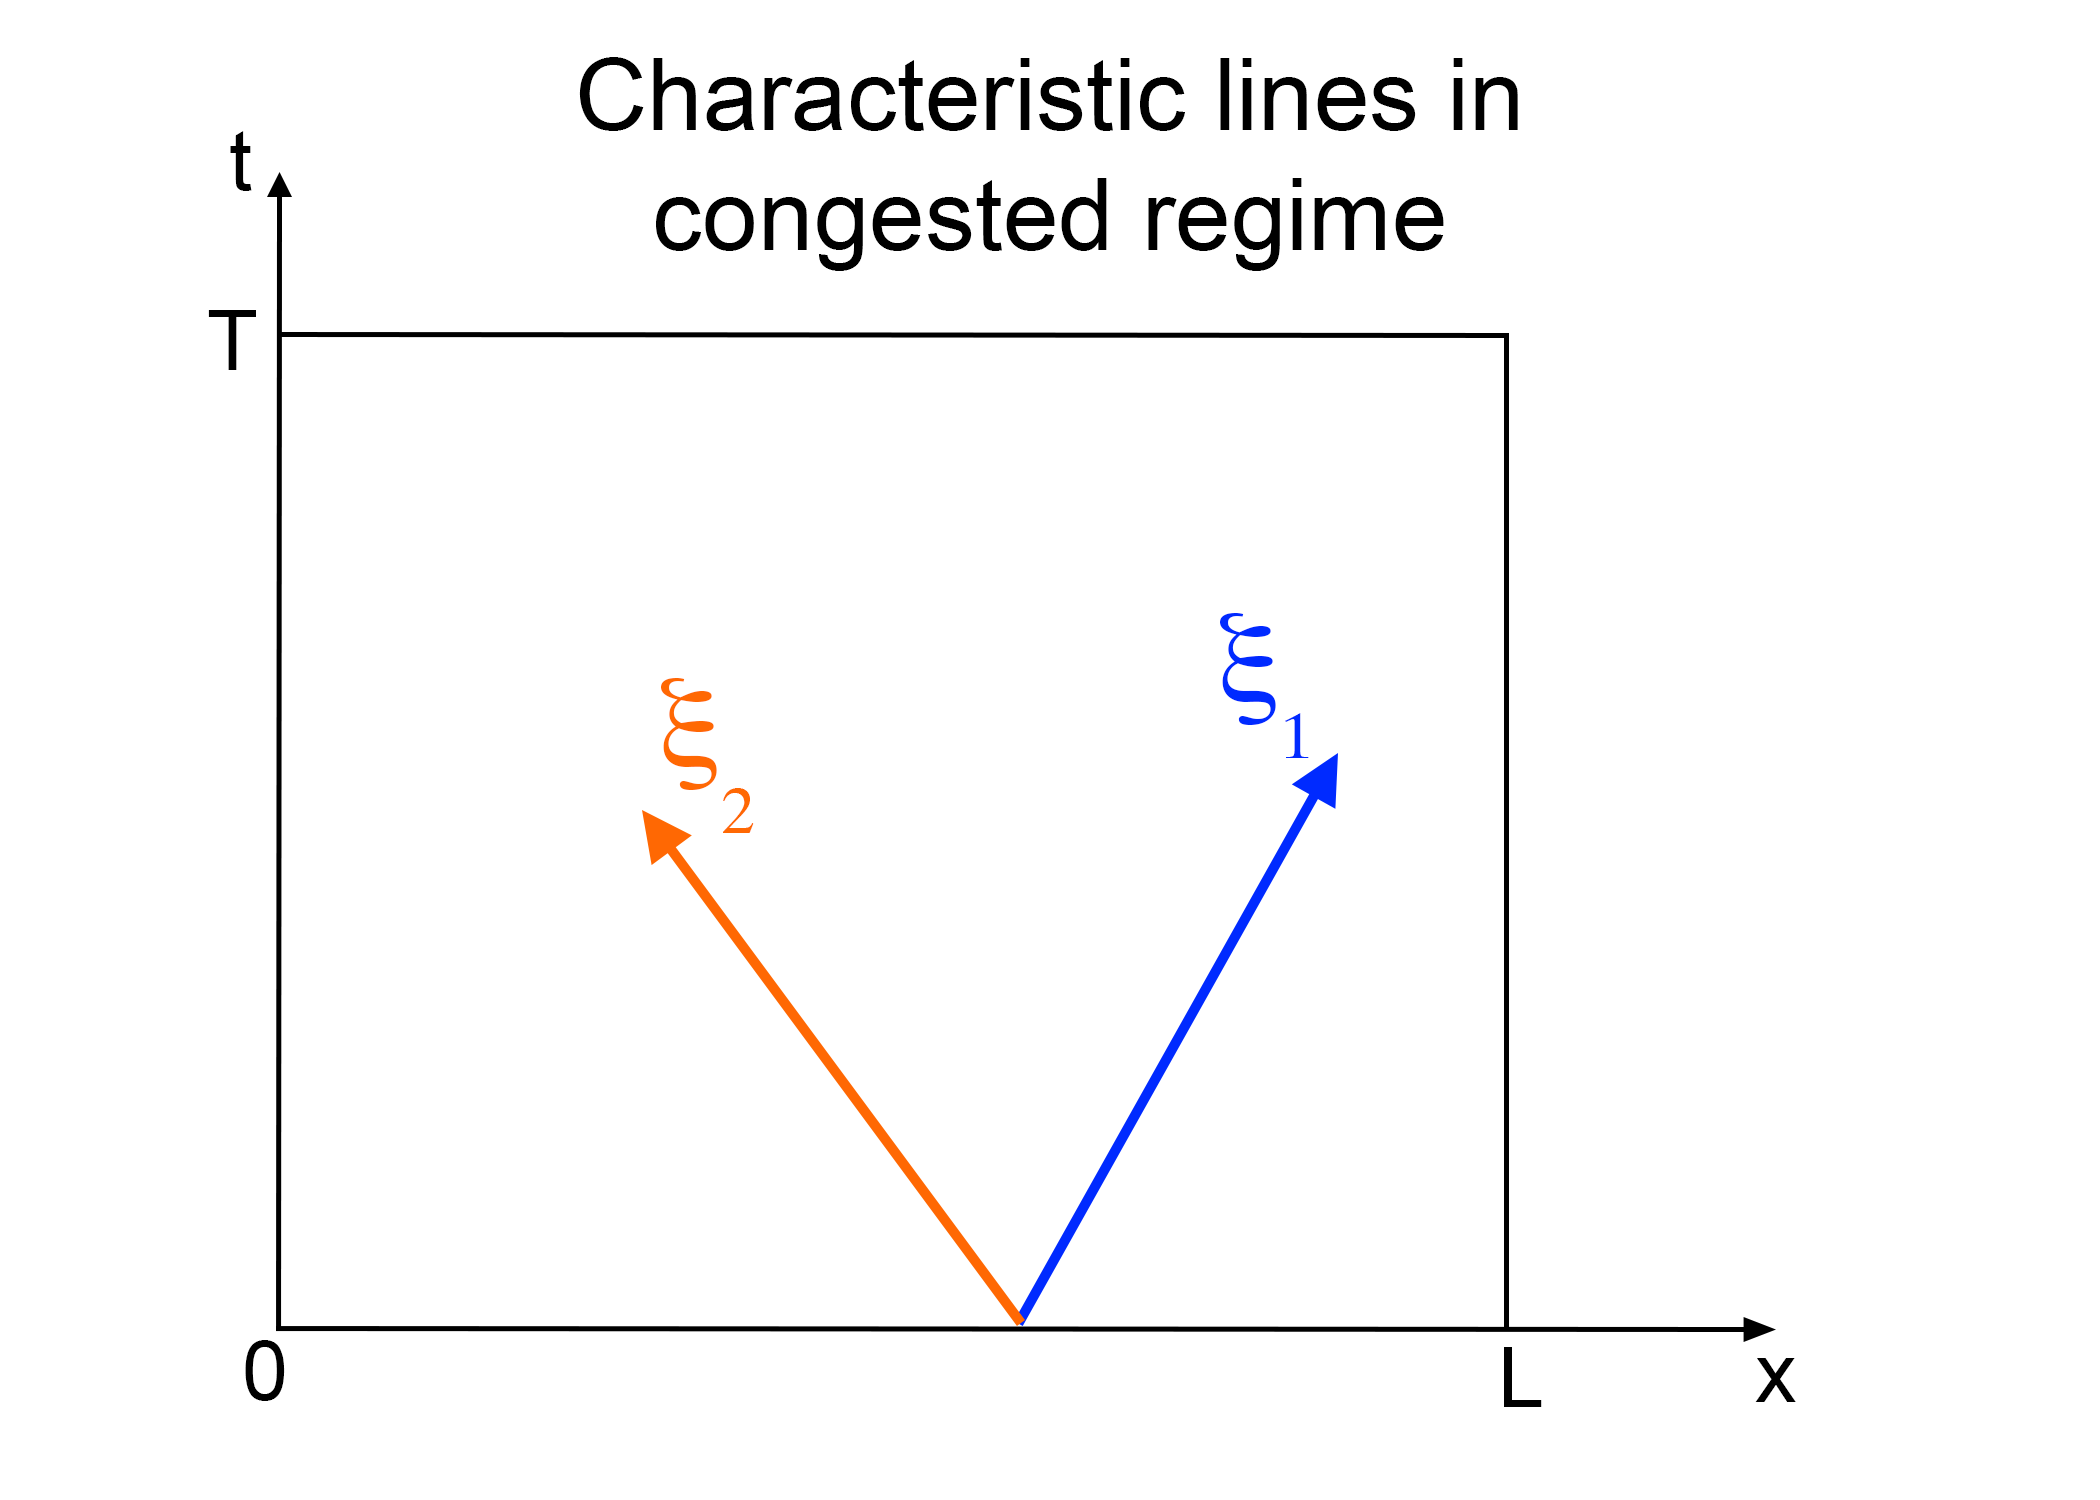
\includegraphics[width=4.5cm]{Congested-regime} & 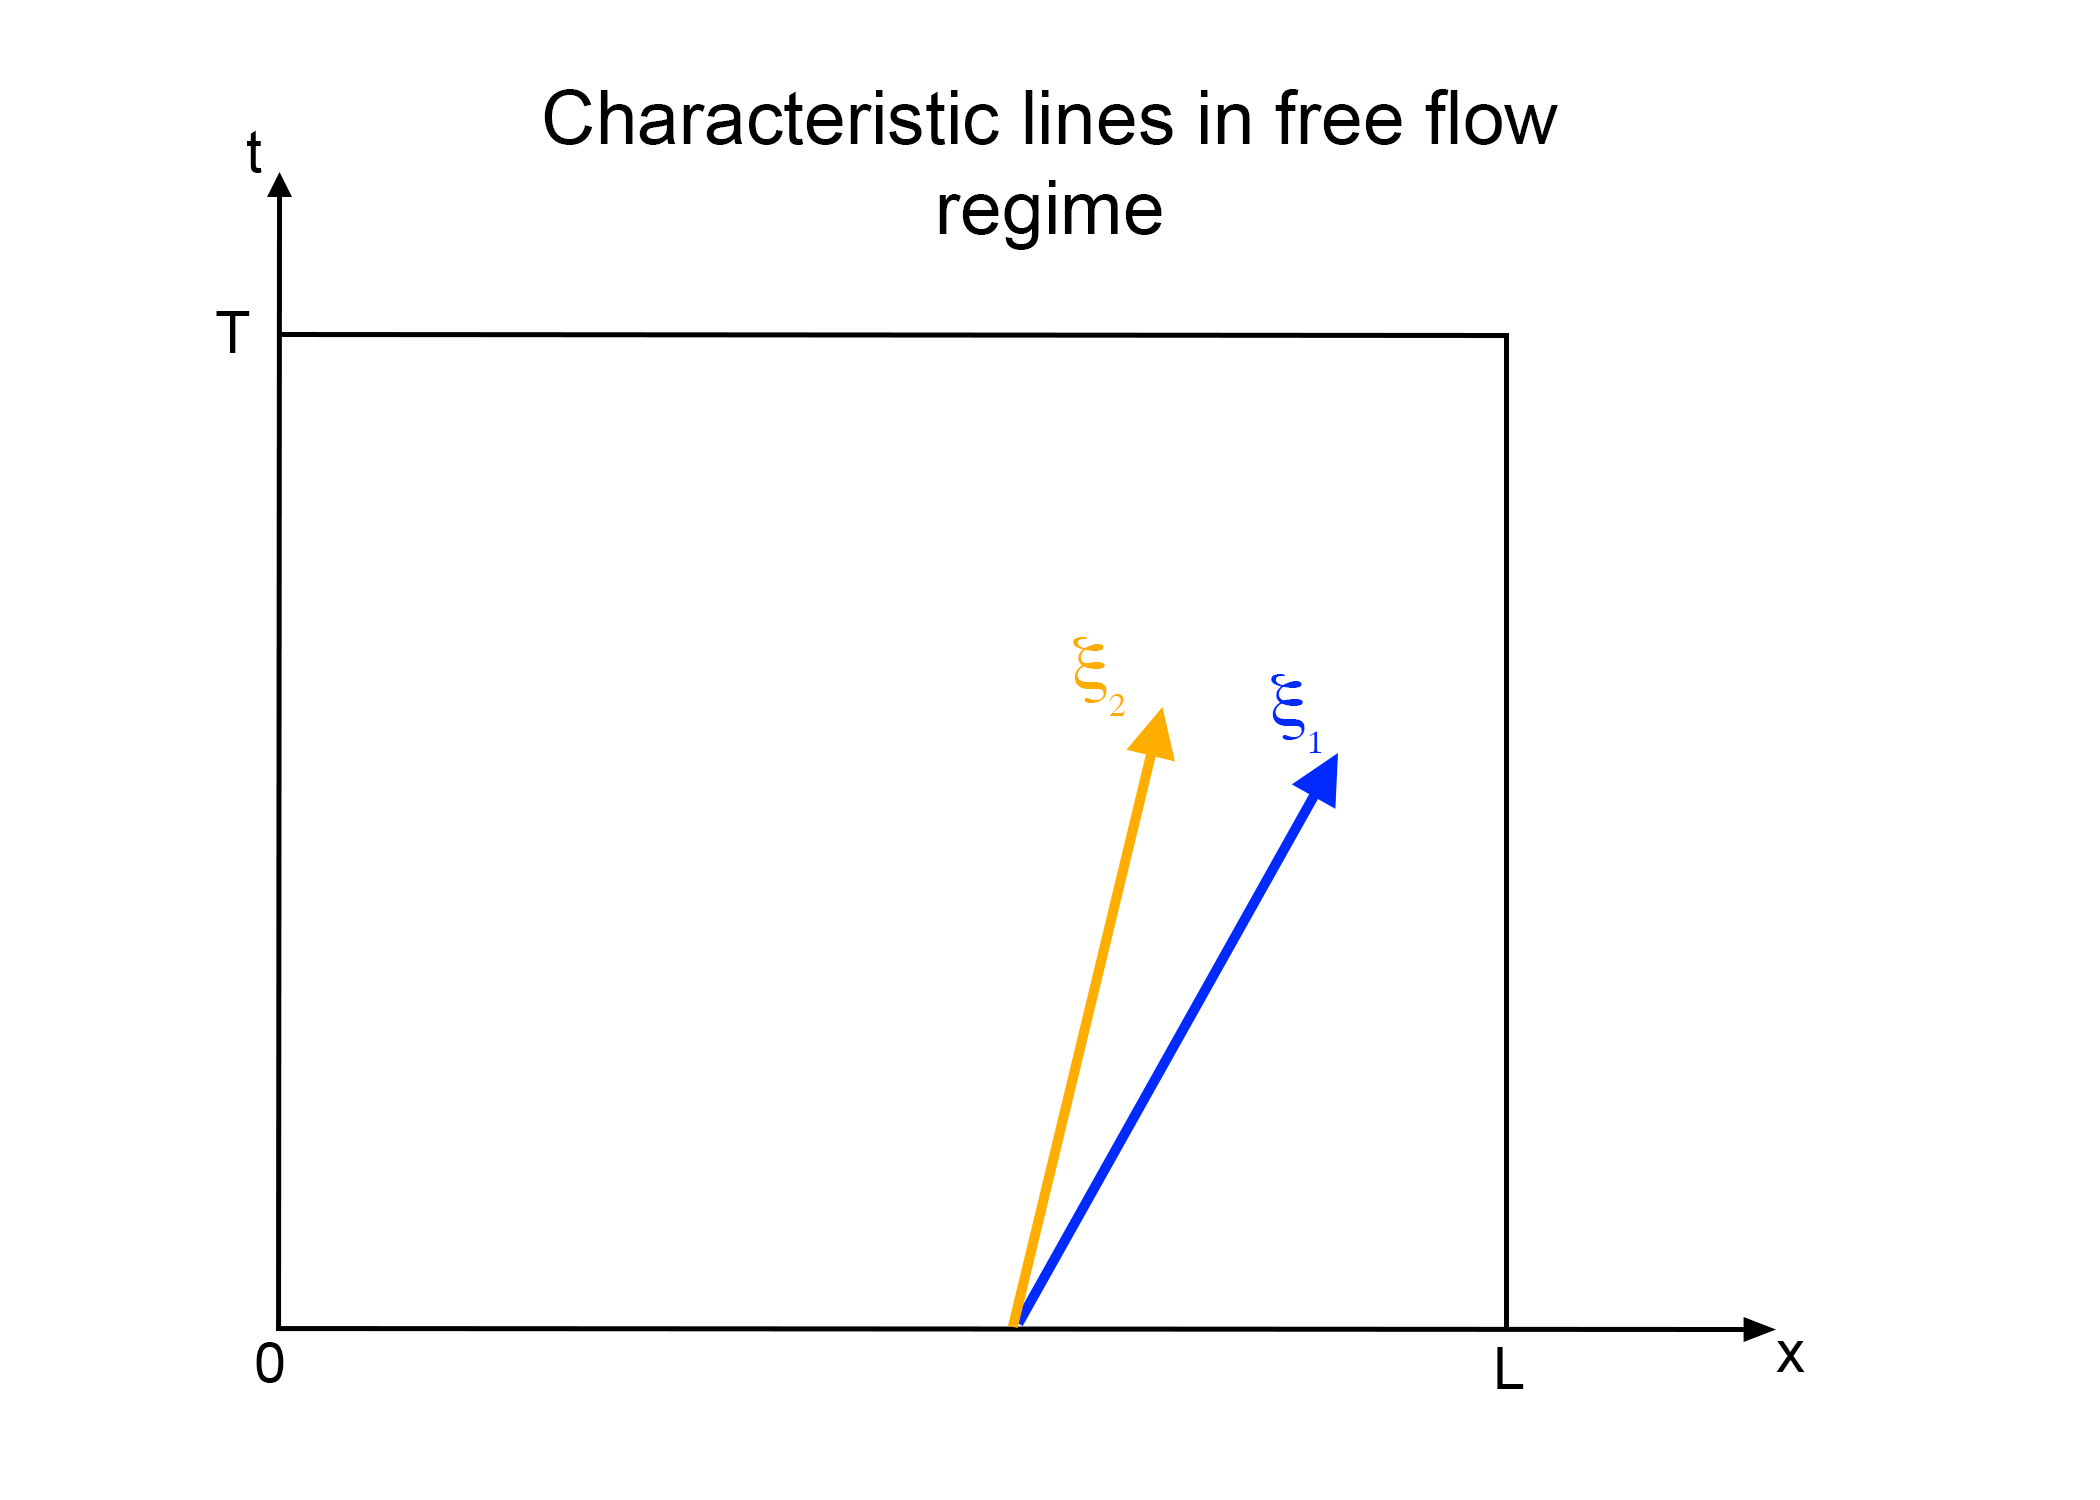
\includegraphics[width=4.5cm]{Free-flow-regime}
\tabularnewline
$F>1$, $\lambda_{2}<0$, $\lambda_{1}>0$ & $F<1$, $\lambda_{1}>\lambda_{2}>0$
\tabularnewline
Inputs $\xi_1(0,t)$ and $\xi_2(L,t)$ &
Inputs $\xi_1(0,t)$ and $\xi_2(0,t)$
\end{tabular}
\par\end{centering}
\protect\caption{Illustration of characteristic lines in congested (supercritical) and free-flow regime (subcritical) $\xi_1$ and $\xi_2$ propagate along.\label{Characteristics}}
\end{figure}


\section{Spectral analysis of the linearized ARZ model}
We now consider the $(v,q)$ system for the frequency domain analysis for practical control purposes.
\subsection{State-transition matrix}
Taking the Laplace transform of the diagonalized form \eqref{vqlindiag} we obtain 
\begin{equation}
\dfrac{\partial \hat{\xi} (x,s)}{\partial x} = \mathscr{A}(s)\hat{\xi}(x,s) + \mathscr{B}\xi(x,t=0^-),
\end{equation}
where $\mathscr{A}(s) = \tilde{A}^{-1}(\tilde{B} - sI)$ and $\mathscr{B} = -\tilde{A}^{-1}$. 
The general solution to this ordinary differential equation is 
\begin{equation}
\hat{\xi}(x,s) = \Phi(x,s)\hat{\xi}(0,s) +  \Phi(x,s) \int^x_0 \Phi(\nu,s)^{-1} \mathscr{B} \xi(\nu,0^-)\text{d} \nu,
\end{equation}
where $\Phi(x,s) = e^{\mathscr{A}(s)x}$ is the state-transition matrix. Assuming zero initial conditions we have 
\begin{equation} \label{TFRiemann}
\hat{\xi}(x,s) = \Phi(x,s)\hat{\xi}(0,s).
\end{equation}

To compute the exponential we diagonalize the matrix as 
\begin{equation}
\mathscr{A}(s) = \mathscr{X}(s)\mathscr{D}(s)\mathscr{X}^{-1}(s)
\end{equation}
where
\begin{equation}
\mathscr{X}(s) = \begin{pmatrix}
0 & \dfrac{\lambda_2 - (\lambda_1 - \lambda_2) \tau s}{\lambda_1} \\
1 & 1
\end{pmatrix},
\mathscr{D}(s) = \begin{pmatrix}
-\frac{s}{\lambda_2} & 0 \\
 0 & -\frac{1+\tau s}{\tau \lambda_1}
\end{pmatrix}.
\end{equation}
Hence
\begin{equation}
\Phi(x,s) =  \mathscr{X}^{-1}(s)e^{\mathscr{D}(s)x}\mathscr{X}(s) =
\begin{pmatrix}
\phi_{11}(x,s) & \phi_{12}(x,s) \\ 
\phi_{21}(x,s) & \phi_{22}(x,s)
\end{pmatrix},
\end{equation}
with
\begin{subequations} \label{TFv0q0tovxqx}
\begin{align}
\phi_{11}(x,s) &= e^{-\frac{x}{\tau \lambda_1}}e^{-\frac{x}{\lambda_1}s}, \\ 
\phi_{12}(x,s) &= 0, \\
\phi_{21}(x,s) &= \dfrac{\lambda_1 \left( e^{-\frac{x}{\tau \lambda_1}}e^{-\frac{x}{\lambda_1}s} - e^{-\frac{x}{\lambda_2}s}\right)}{\lambda_2 - \tau (\lambda_1 - \lambda_2)s}, \\
\phi_{22}(x,s) &= e^{-\frac{x}{\lambda_2}s}.
\end{align}
\end{subequations}



Let $\alpha = -\dfrac{\lambda_2}{\tau(\lambda_1 - \lambda_2)}$. It is clear that $\phi_{11}\left(x,s\right)$ is composed of the product of a distributed delay corresponding to information propagating at speed $\lambda_{1}$ and an exponential attenuation where $\tau\lambda_{1}$ plays the role of a characteristic spatial length. Similarly $\phi_{22}$ is a delay corresponding to information propagating at speed $\lambda_{2}$. The interpretation of $\phi_{21}$ is more difficult. In low frequencies ($\left|s\right|\ll\left|\alpha\right|$), this transfer function takes a much more transparent form. Indeed, in the expression
$
\phi_{21}(x,s) = 
-\frac{\lambda_{1}}{\lambda_{2}}\frac{\alpha}
{s + \alpha}
e^{-\frac{x}{\lambda_2}s}
	\left(
		1 - e^{-\frac{x}{\lambda_1 \tau \alpha}\left(s + \alpha\right)}
	\right)
\simeq 
- \frac{\lambda_{1}}{\lambda_{2}} e^{-\frac{x}{\lambda_2}s}
	\left(
		1 - e^{-\frac{x}{\lambda_1 \tau}}
	\right)
$
the transfer function appears as the combination of a distributed delay where $\lambda_{2}$ is the propagation speed and a distributed gain where $\lambda_{1}\tau$ is a characteristic distance.

\subsection{Free-flow case ($F<1$)}
Consider the system in the free-flow regime. With $\xi_1 (0,t)$ and $\xi_2 (0,t)$ as the inputs and $\xi_1(L,t)$ and $\xi_2(L,t)$ as the outputs, the distributed transfer matrix is exactly the state-transition matrix $\Phi(x,s)$. Using \eqref{eq:Riemannzeta}, we can write

\begin{equation} \label{vqfreeflow}
\begin{pmatrix}
\widetilde{v}(x,s) \\ \widetilde{q}(x,s)
\end{pmatrix} = \underbrace{ \begin{pmatrix}
\dfrac{\rho^*\lambda_2}{\lambda_1-\lambda_2} & 1\\
\dfrac{\rho^*\lambda_1}{\lambda_1-\lambda_2} & 0
\end{pmatrix}^{-1} \Phi(x,s) 
\begin{pmatrix}
\dfrac{\rho^*\lambda_2}{\lambda_1-\lambda_2} & 1\\
\dfrac{\rho^*\lambda_1}{\lambda_1-\lambda_2} & 0
\end{pmatrix} }_\text{$\Psi (x,s)$} \begin{pmatrix}
\widetilde{v}(0,s) \\ \widetilde{q}(0,s)
\end{pmatrix}
\end{equation}
with
\begin{subequations}
\label{psis}
\begin{align}
\psi_{11}(x,s) &= 
\frac{
	\alpha e^{-\frac{x}{\lambda_{1}}\left(s+\frac{1}{\tau}\right)}
		+ s e^{-\frac{sx}{\lambda_{2}}}
}{
	s + \alpha
}, \\
\psi_{12}(x,s) &=
\frac{1}{\rho^* \tau}
\frac{
	e^{-\frac{sx}{\lambda_{2}}}
	-
	e^{-\frac{x}{\lambda_{1}}\left(s+\frac{1}		{\tau}\right)}
}{
	s + \alpha
}, \\
\psi_{21}(x,s) &=
- s \rho^{*} \tau \alpha
\frac{
	e^{-\frac{sx}{\lambda_{2}}}
	-
	e^{-\frac{x}{\lambda_{1}}\left(s+\frac{1}		{\tau}\right)}
}{
	s + \alpha
}, \\
\psi_{22}(x,s) &=
\frac{
	s e^{-\frac{x}{\lambda_{1}}\left(s+\frac{1}{\tau}\right)}
		+ \alpha e^{-\frac{sx}{\lambda_{2}}}
}{
	s + \alpha
}.
\end{align}
\end{subequations}

It could appear at first sight that $-\alpha$ (here a positive real) is a singularity of the transfer functions and the system is not bounded-input/bounded-output stable. However, we have $\frac{1}{\lambda_{1}}\left(-\alpha+\frac{1}{\tau}\right)=\frac{1}{\tau\left(\lambda_{1} - \lambda_{2}\right)}=\frac{-\alpha}{\lambda_{2}}$, thus a Taylor expansion about $-\alpha$ shows that numerators and denominators cancel each other out for $s \rightarrow -\alpha$. It follows that $-\alpha$ is not a pole of any transfer function. 
The spectrum of $\Psi(x,s)$ is identical to that of $\Phi(x,s)$ which is lower triangular and has eigenvalues 
$
e^{ - \frac{x}{\tau \lambda_1}}
e^{ - \frac{x}{\lambda_1} s}
$
and
$
e^{ - \frac{x}{\lambda_2} s}
$
whose module is trivially bounded by $1$.
This proves the $H_{\infty}$ norm of $\Psi$ is $1$ and therefore the system is Bounded-Input/Bounded-Output (BIBO) stable. This proves that the output remains bounded for a given value of $x$. 

We will show below that a conic region of the $\left[0,T\right] \times \left[0,L\right]$ domain features exponential growth in free-flow regime. This arises when changing $t$ and $x$ simultaneously and complements the conclusion formulated above (in which $t$ varies and $x$ remains constant).

\subsubsection{Low frequency approximation for physical variables in free-flow regime}
Analyzing the expressions above becomes easier when approximating them for $\left|s\right|\ll\left|\alpha\right|$. This corresponds to traffic flow varying slowly and smoothly. We find the following approximate expressions for the transfer functions:
\begin{subequations}
\begin{align}
\psi_{11}(x,s)
&\simeq
e^{-\frac{sx}{\lambda_{2}}}
e^{-\frac{x}{\tau\lambda_{1}}}
, \\
\psi_{12}(x,s)
&\simeq
\frac{
	1
}{
	\rho^{*}\tau\alpha
}
e^{-\frac{sx}{\lambda_{2}}}
\left(
	1 - e^{-\frac{x}{\tau\lambda_{1}}}
\right)
, \\
\psi_{21}(x,s)
& \simeq
- s \rho^{*} \tau
e^{-\frac{sx}{\lambda_{2}}}
\left(
	1 - e^{-\frac{x}{\tau\lambda_{1}}}
\right)
, \\
\psi_{22}(x,s)
&\simeq
e^{-\frac{sx}{\lambda_{2}}}
.
\end{align}
\end{subequations}

Interpreting the low frequency expressions is fairly straightforward.
In $\psi_{11}$, $e^{-\frac{sx}{\lambda_{2}}}$ is a distributed delay with propagation speed $\lambda_{2}$ and $e^{-\frac{x}{\tau\lambda_{1}}}$ a distributed gain with characteristic distance $\tau\lambda_{1}$. 
In $\psi_{12}$ and $\psi_{21}$ we can notice the combination of a distributed delay whose  characteristic speed is $\lambda_{2}$ and a distributed gain whose characteristic distance is $\tau\lambda_{1}$. It is also remarkable that $\widetilde{q}(x,s)$ appears as the result of a derivator applied to $\widetilde{v}(0,s)$.
The approximate expression for $\psi_{22}$ highlights the presence of a distributed delay where information propagates at speed $\lambda_{2}$.

\subsubsection{Bode plots for free-flow regime}

We generate Bode plots using the following parameters taken from \cite{Hofleitner}: $q_{\text{max}}$ = 1300 veh/h, $\rho_{\text{max}}$ = 0.1 veh/m, and $L$ = 100 m. The Greenshields fundamental diagram, where the equilibrium flow is $Q(\rho) = 4 \frac{q_{\text{max}}}{\rho_{\text{max}}^2}\rho (\rho_{\text{max}} - \rho)$, is used to approximate the fundamental diagram. For inhomogeneous second-order models, the relaxation time, $\tau$, falls in the range of about 14-60 seconds \cite{Fan}. A relaxation time of $\tau$ = 15 s is used for the following simulations. We simulate for $\rho^* = 0.01$ veh/m. Here the characteristic frequency of the system, $\left|\alpha\right|$, equals 0.53 Hz which is indeed sensible for traffic flow modeling.

The Bode plots for the physical variables are displayed in Figure \ref{fig:Magn_spatial_physx}.
For the Riemann invariants only $\phi_{21}(x,s)$ and $\phi_{22}(x,s)$ are represented in Figure \ref{fig:Magn_spatial_diag} ($\phi_{11}(x,s)$ and $\phi_{12}(x,s)$ are only delay functions).

\begin{figure}
\centering
\begin{tabular}{cc}
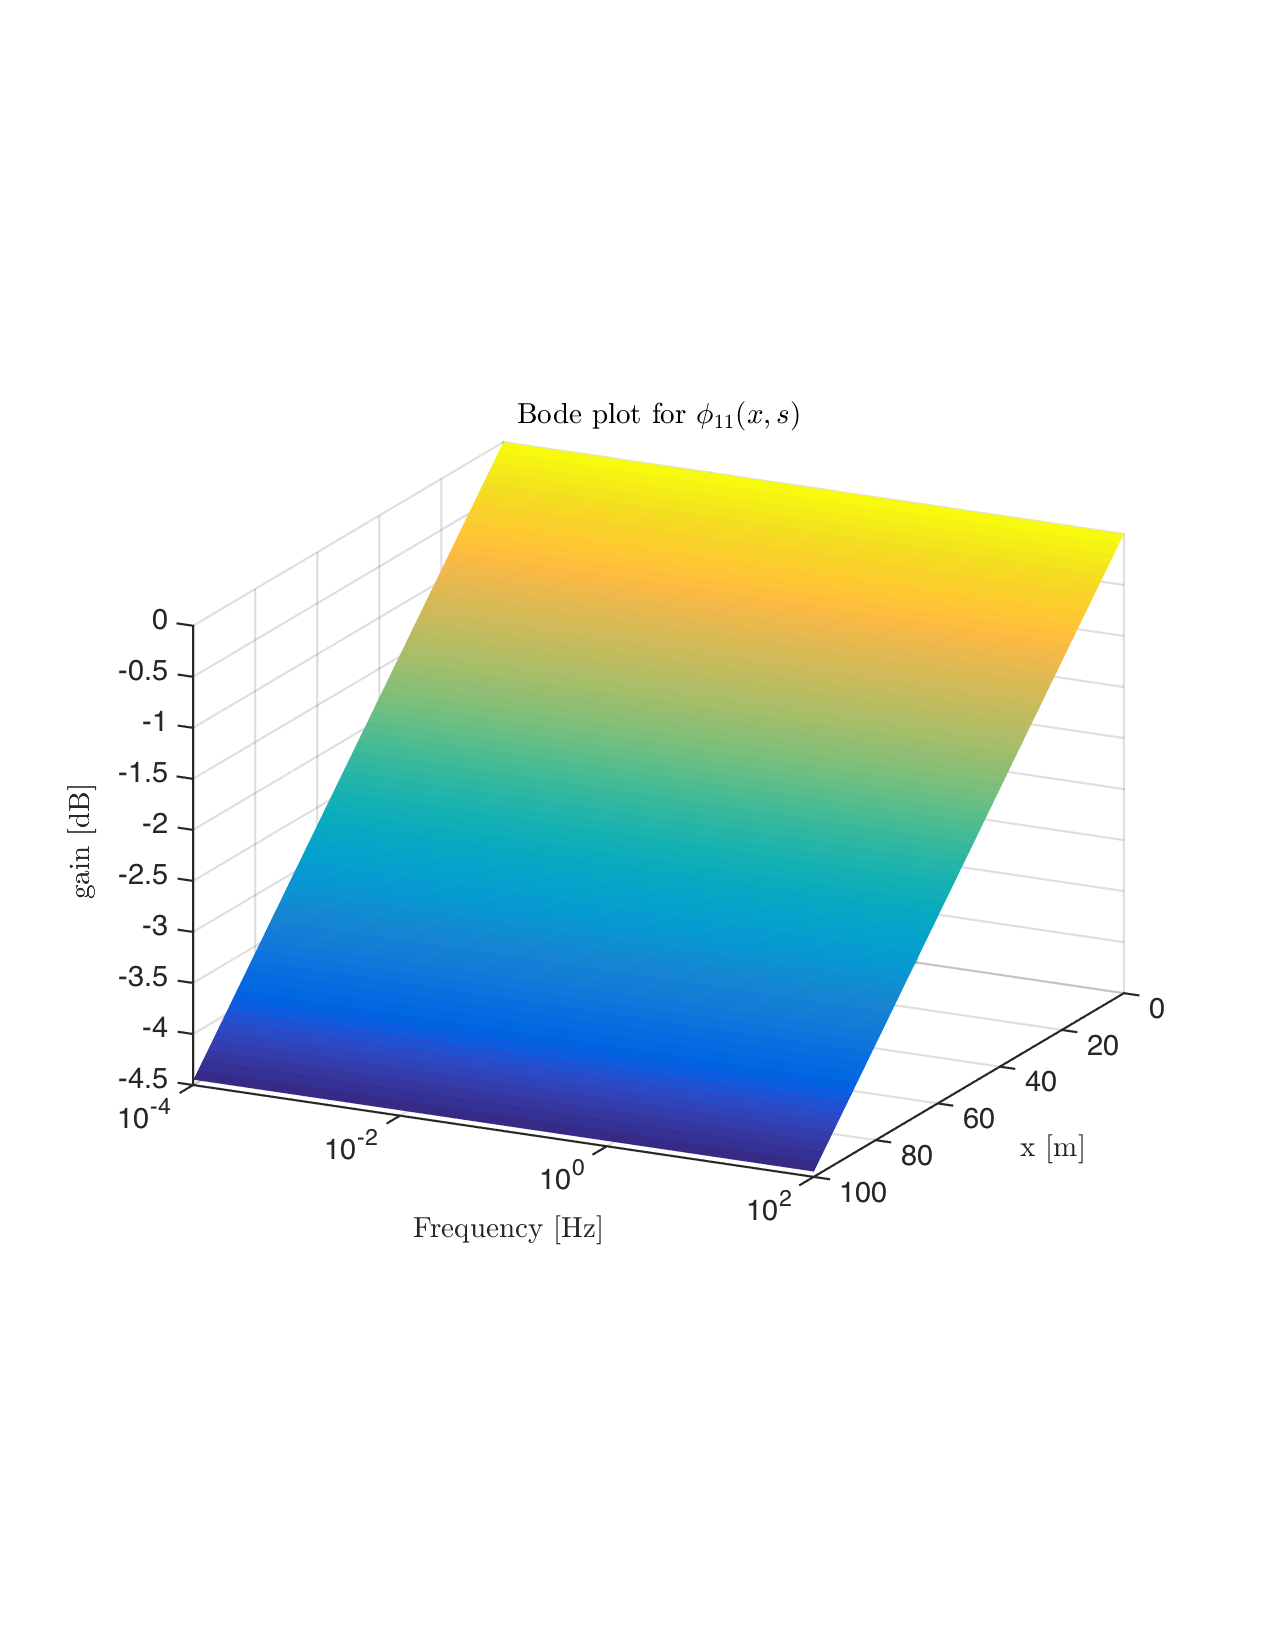
\includegraphics[trim = 0mm 60mm 0mm 60mm, width = 4.2cm]{distr_phi_11}
&
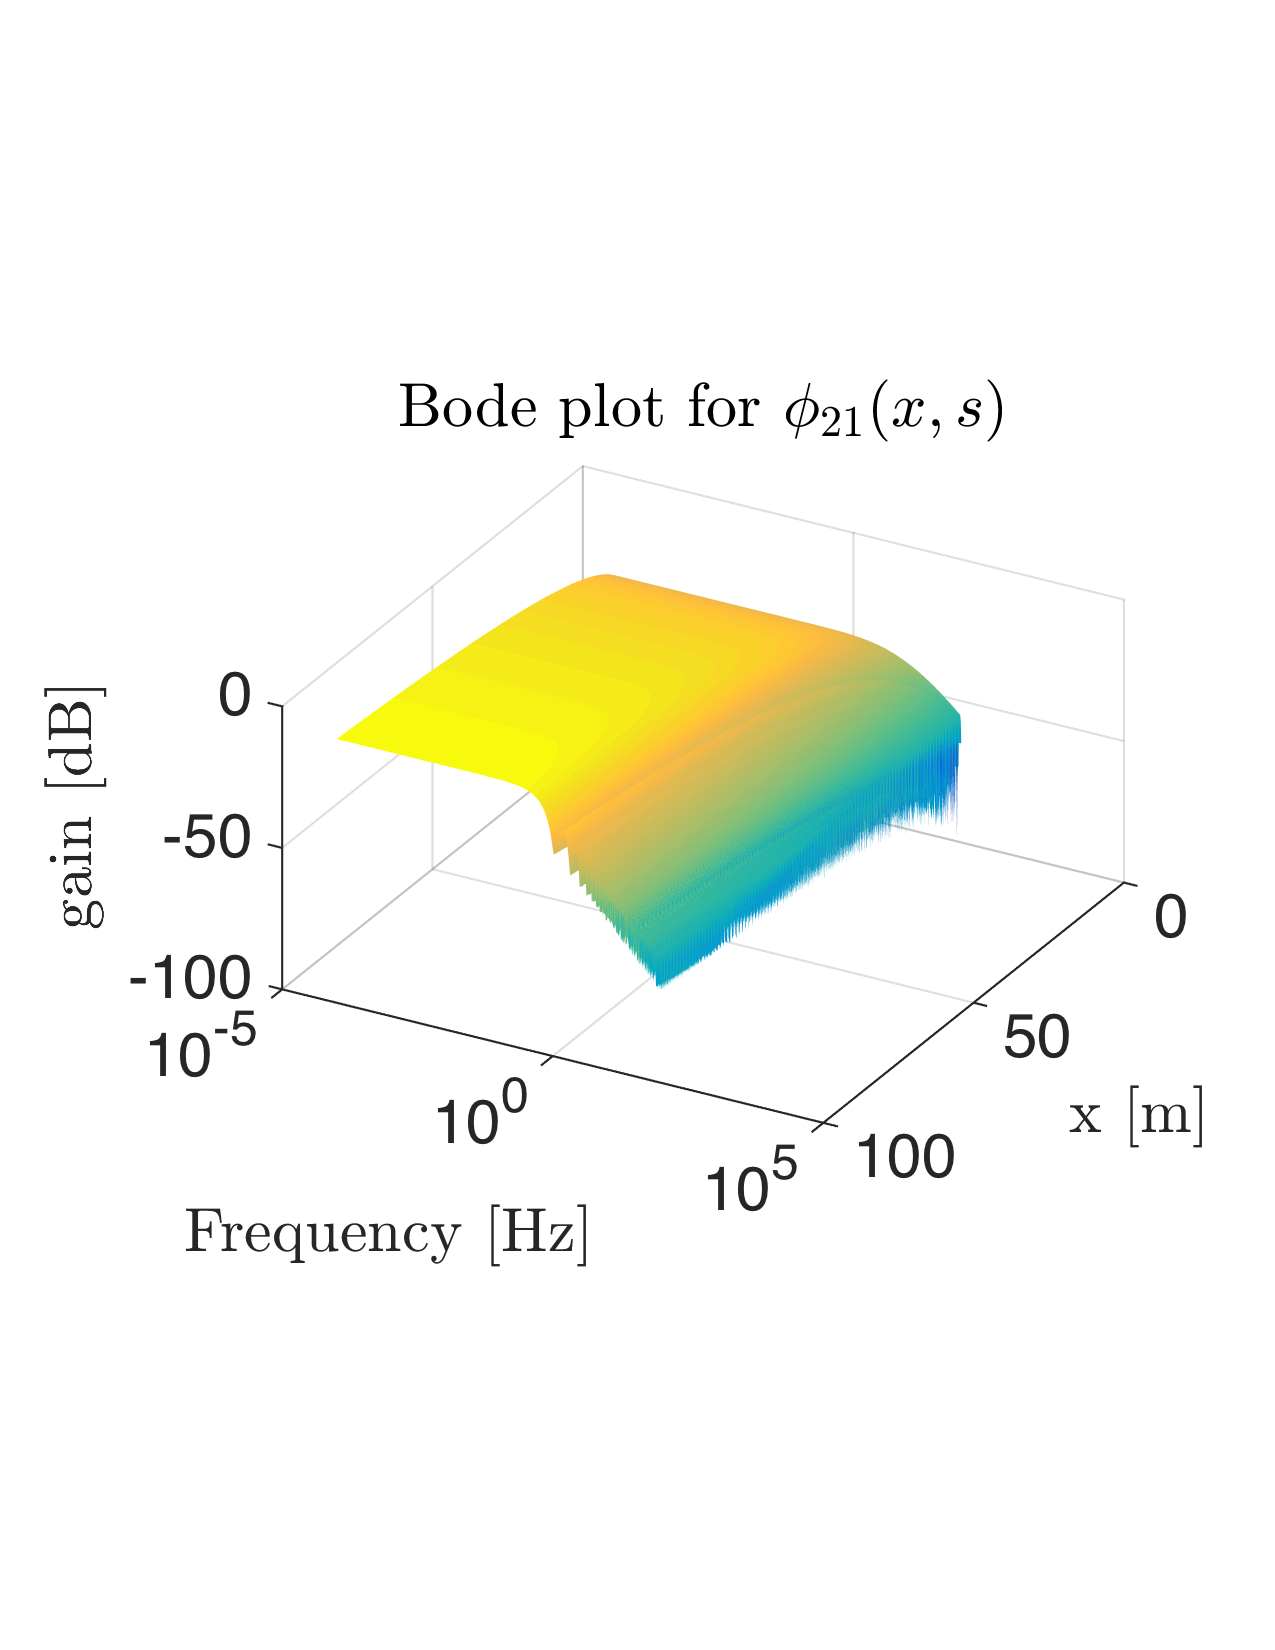
\includegraphics[trim = 0mm 60mm 0mm 60mm, width = 4.2cm]{distr_phi_21}
\tabularnewline
Bode plot for $\phi_{11}(x,s)$.
&
Bode plot for $\phi_{21}(x,s)$.
\tabularnewline

\end{tabular}
\caption{Spatial magnitude Bode plots for Riemann invariants in free-flow regime ($\left|\alpha\right| = $ 0.53 Hz)\label{fig:Magn_spatial_diag}}
\end{figure}

\begin{figure}
\centering
\begin{tabular}{cc}
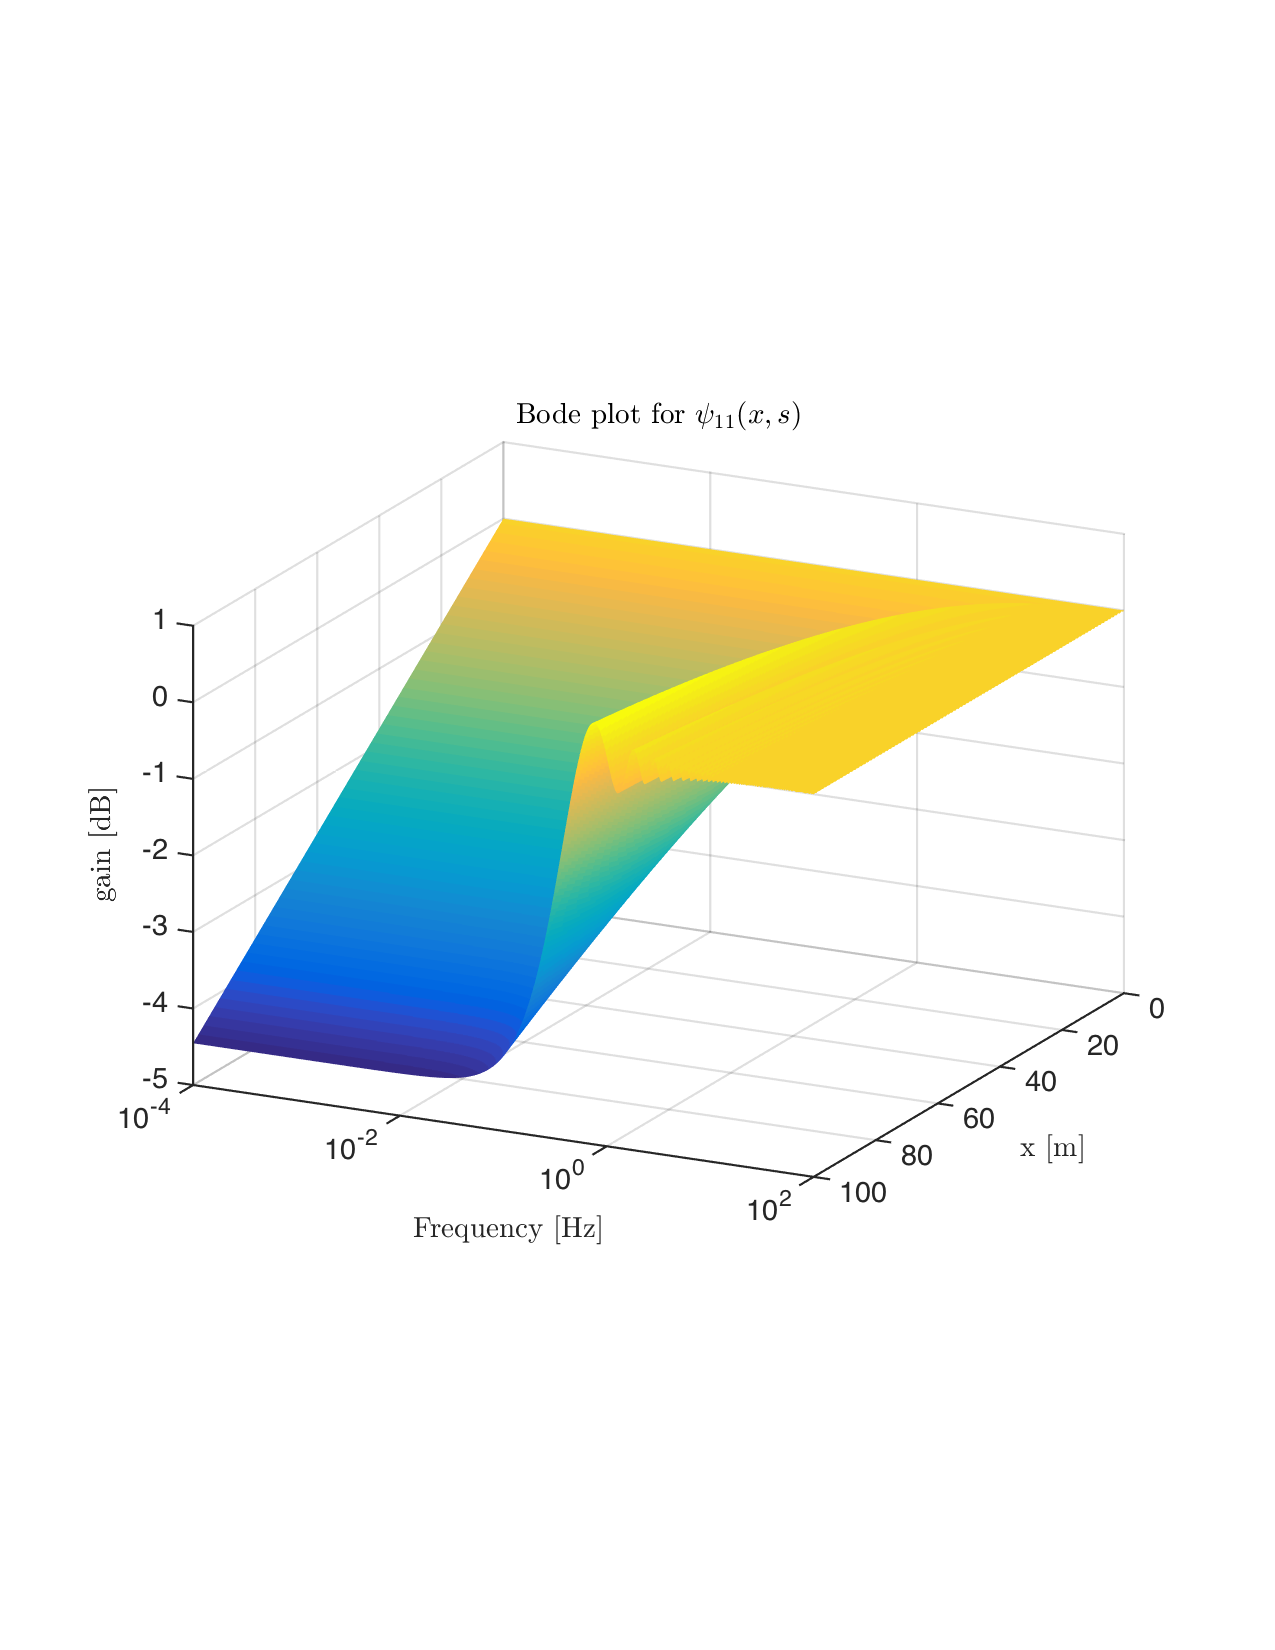
\includegraphics[trim = 0mm 60mm 0mm 60mm, width = 4.2cm]{distr_psi_11}
&
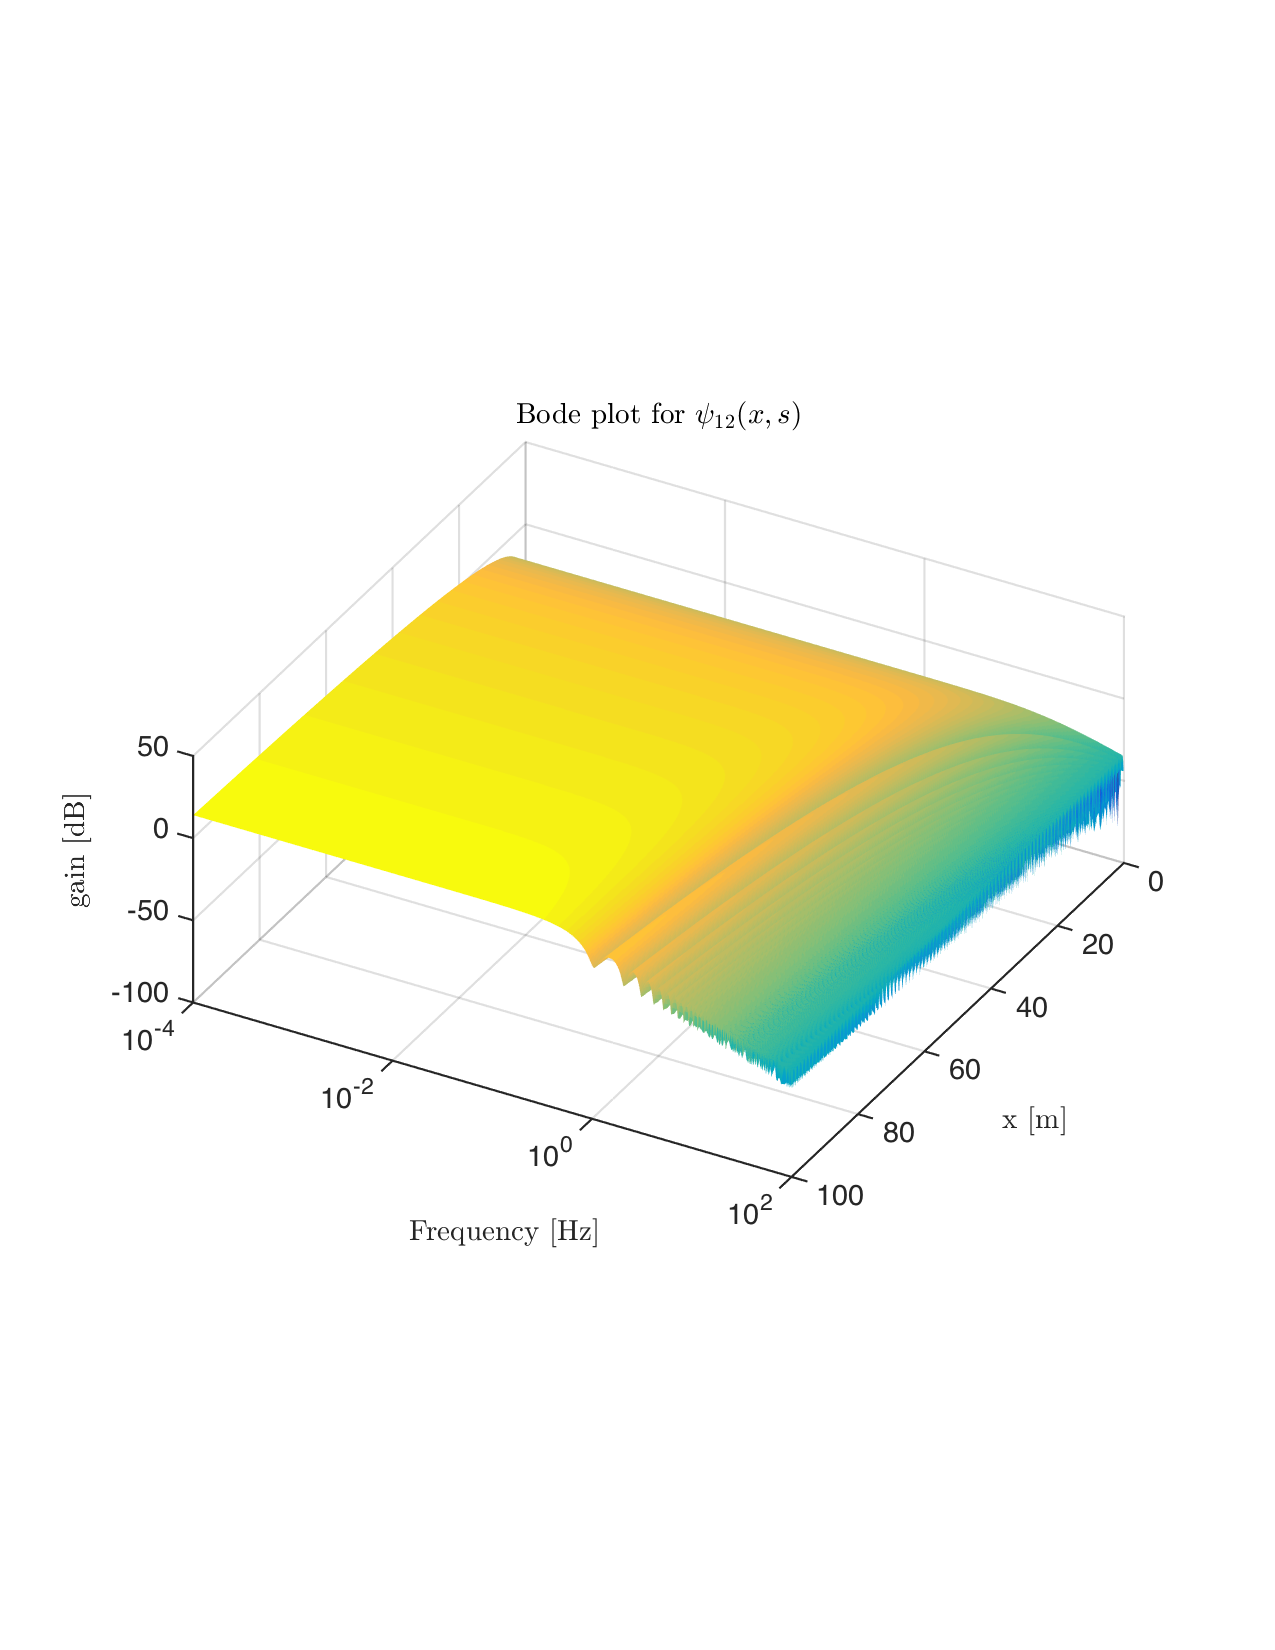
\includegraphics[trim = 0mm 60mm 0mm 60mm, width = 4.2cm]{distr_psi_12}
\tabularnewline
Bode plot for $\psi_{11}(x,s)$.
&
Bode plot for $\psi_{12}(x,s)$.
\tabularnewline
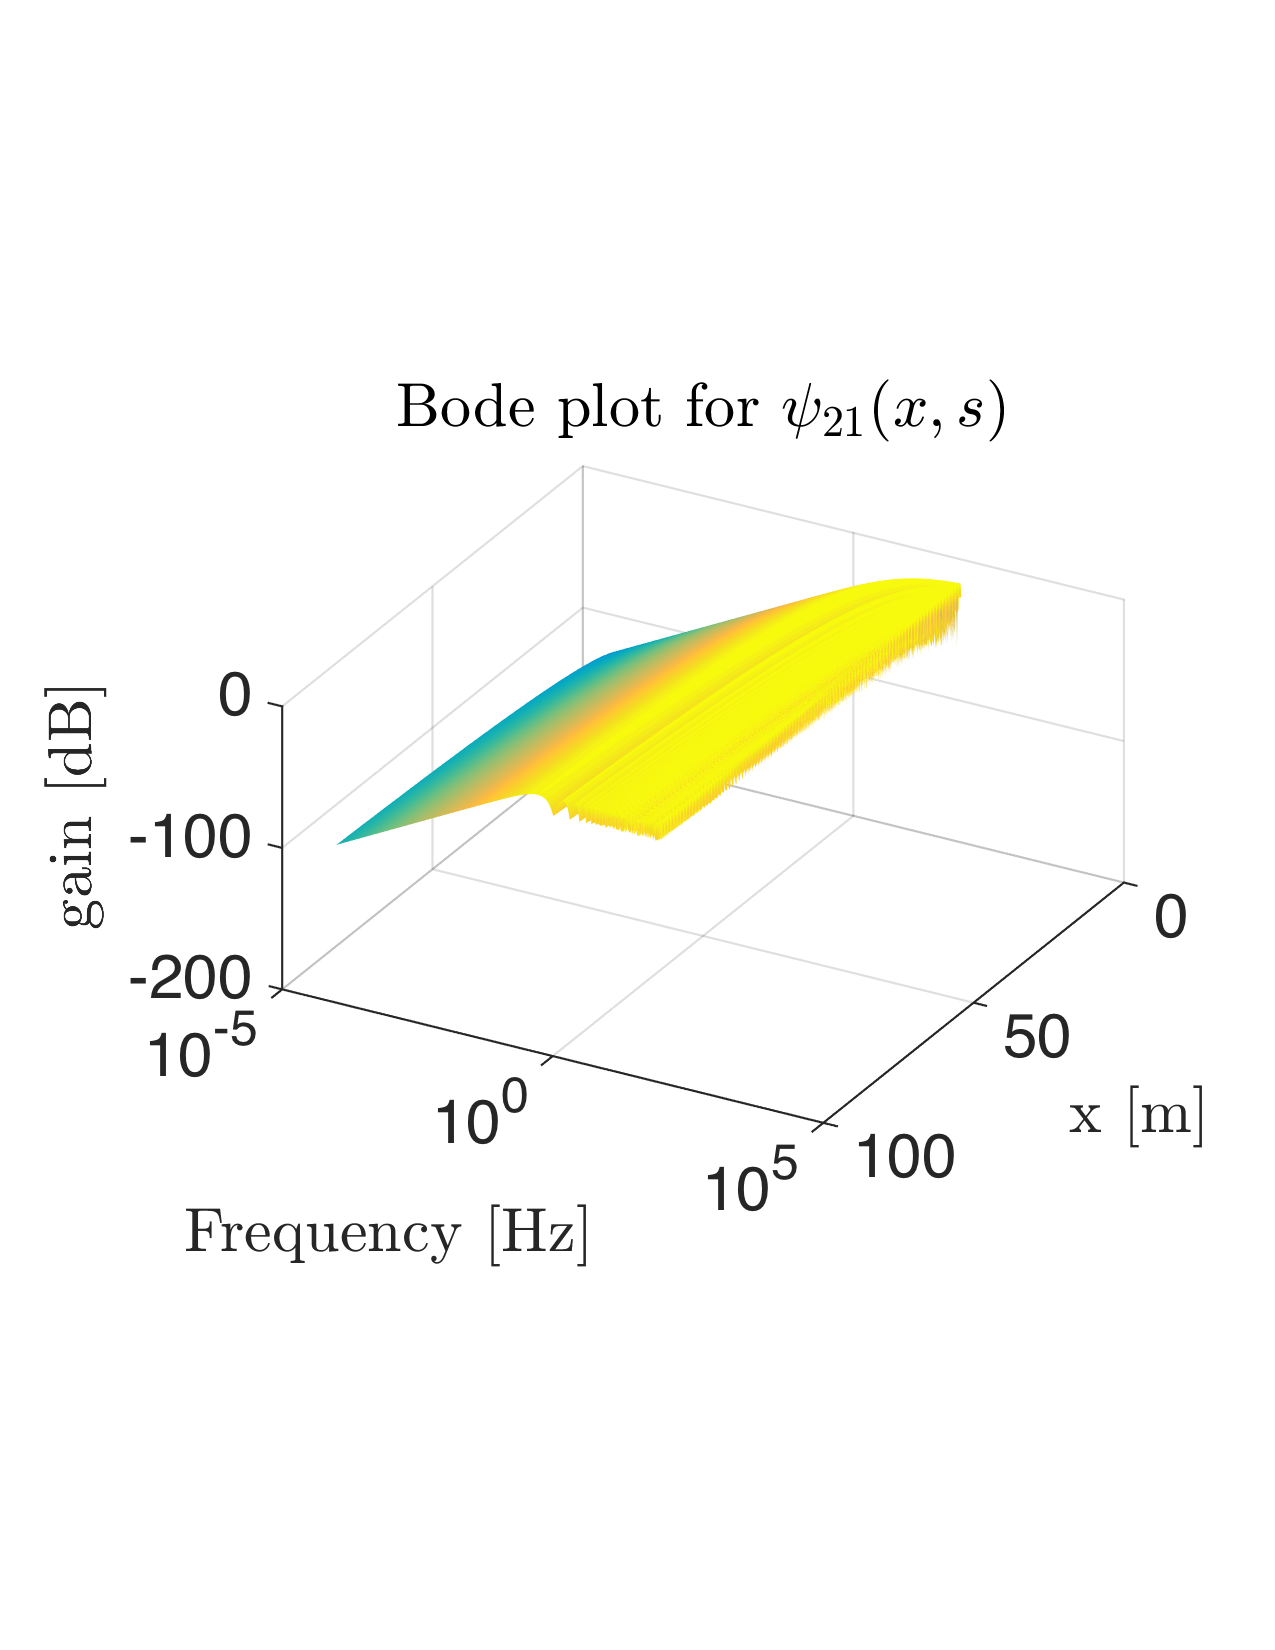
\includegraphics[trim = 0mm 60mm 0mm 60mm, width = 4.2cm]{distr_psi_21}
&
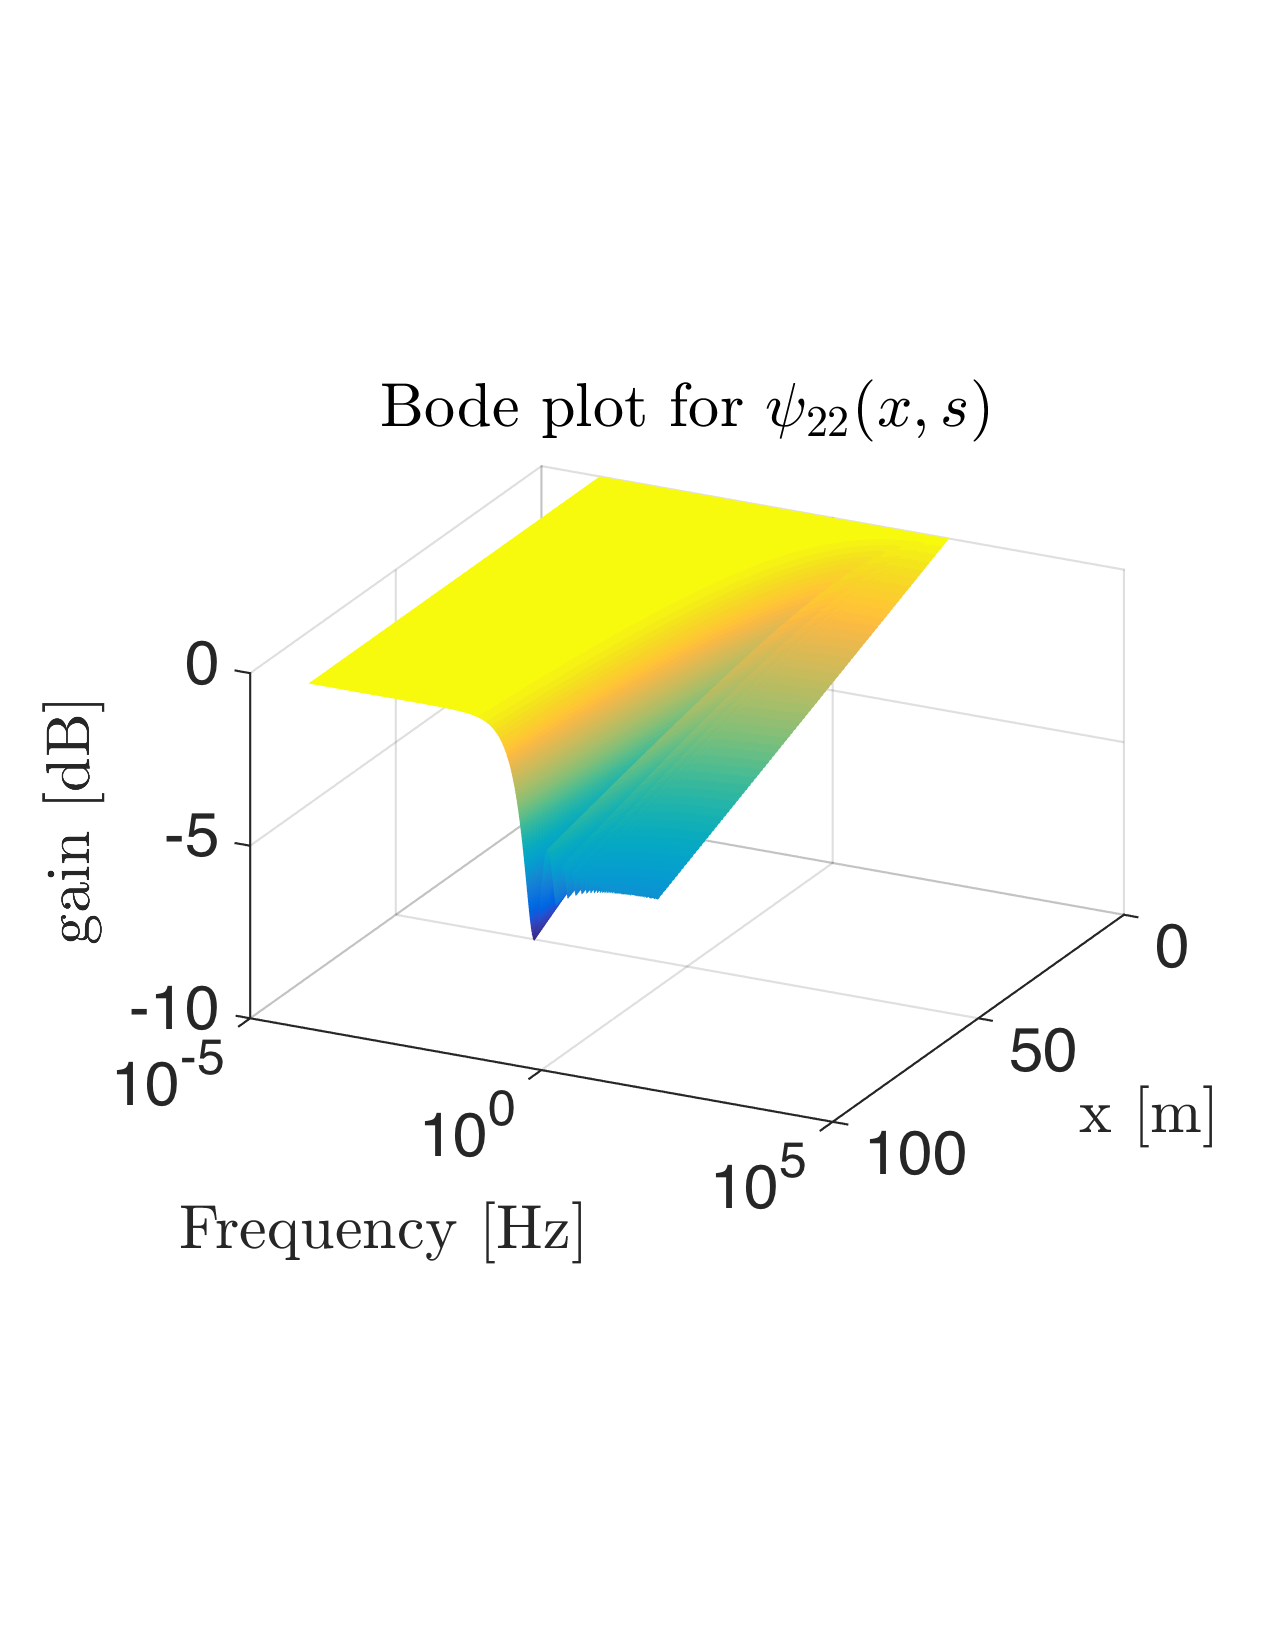
\includegraphics[trim = 0mm 60mm 0mm 60mm, width = 4.2cm]{distr_psi_22}
\tabularnewline
Bode plot for $\psi_{21}(x,s)$.
&
Bode plot for $\psi_{22}(x,s)$.
\tabularnewline
\end{tabular}
\caption{Spatial magnitude Bode plots for physical variables in free-flow regime ($\left|\alpha\right| = $ 0.53 Hz)\label{fig:Magn_spatial_physx}}
\end{figure}

For transfer functions featuring $1 - e^{-\frac{x}{\lambda_{1} \tau \alpha} \left(s + \alpha \right)}$ as a factor (that is to say $\phi_{21}$, $\psi_{12}$, and $\psi_{21}$) one can observe in the corresponding Bode plots that the value of the log-gain in high frequency tends to vary very sharply. Indeed, with $s = jw$,
$
\left| 
	1 - e^{-\frac{x}{\lambda_{1} \tau \alpha} \left(s + \alpha\right)}
\right| = 
e^{-\frac{x}{\lambda_{1} \tau}}
\sqrt{
	\left(
		e^{\frac{x}{\lambda_{1}\tau}} 
		-
		\cos\left(\frac{w}{\lambda_{1} \tau \alpha} x\right)
	\right)^{2}
	+
	\sin^{2}\left( \frac{w}{\lambda_{1} \tau \alpha} x \right)
}
$. Therefore, if the spatial pseudo-period $\tilde{L}=\frac{2\pi}{w} \lambda_{1} \tau \left|\alpha\right|$ is low enough, near zero values appear when $x$ is a multiple of $\tilde{L}$. This explains the irregular shape of the distributed Bode plots of $\phi_{21}$, $\psi_{12}$, and $\psi_{21}$ for frequencies $w \gg 2 \pi \frac{\lambda_{1} \tau \left|\alpha\right|}{L} = 6.53$ Hz. This does not impact the stability of the system. Bode plots only look irregular about such points because of the logarithmic scale.

\subsubsection{Step responses}
We analyze the behavior of the system given step inputs $\tilde{v}(0,t)=v_{\text{step}}H(t)$ and $\tilde{q}(0,t)=q_{\text{step}}H(t)$, where $H(\cdot)$ is the Heaviside function. The step responses can be explicitly computed from the spectral responses. Letting $H_1(t,x) = H\left(t-\frac{x}{\lambda_{1}}\right)$ and
$H_2(t,x) = H\left(t - \frac{x}{\lambda_{2}} \right)$:
\begin{align}
\tilde{v}(x,t) &= 
\bar{v}
e^{-\frac{x}{\lambda_{1}\tau}}H_1(t,x)
\notag\\
&\quad
+\bar{v}
e^{-\alpha \left(t - \frac{x}{\lambda_{2}} \right)}
	(H_2 - H_1)(t,x)
\notag \\
&\quad
- \dfrac{\bar{q}}{\rho^* \tau}
\left(
	e^{-\frac{x}{\lambda_{1}\tau}}H_1\left(t,x\right) 
	- H_2(t,x)
\right) 
\notag\\
&\quad
- \dfrac{\bar{q}}{\rho^* \tau} e^{-\alpha \left(t - \frac{x}{\lambda_{2}} \right)}
	(H_2 - H_1)(t,x)\\
\tilde{q}(x,t) &= \bar{v} \rho^*\tau \alpha e^{-\alpha \left(t - \frac{x}{\lambda_{2}} \right)}
	(H_1 - H_2)(t,x)
\notag \\
&\quad+ 
\bar{q}
H_2(t,x)
\notag\\
&\quad
+
\bar{q}
e^{-\alpha \left(t - \frac{x}{\lambda_{2}} \right)}
	(H_1 - H_2)(t,x)	
\end{align}

With this set of time domain expressions, we can see that a cone of exponentially growing speed and flow linearization errors generally appears between the characteristic lines corresponding to $\lambda_{1}$ and $\lambda_{2}$. This is caused by $\alpha$ being negative in the free flow regime and means that, in this region of the domain $\left[0,T\right] \times \left[0,L\right]$, the $\left(v,q\right)$ state of the linearized system can diverge exponentially fast from the linearization point. This is consistent with the observations in \cite{PhysRevLett.79.4030} where small local perturbations occurring in free-flow regime can cause traffic to transition durably to the congested regime.

\begin{figure}
\begin{centering}
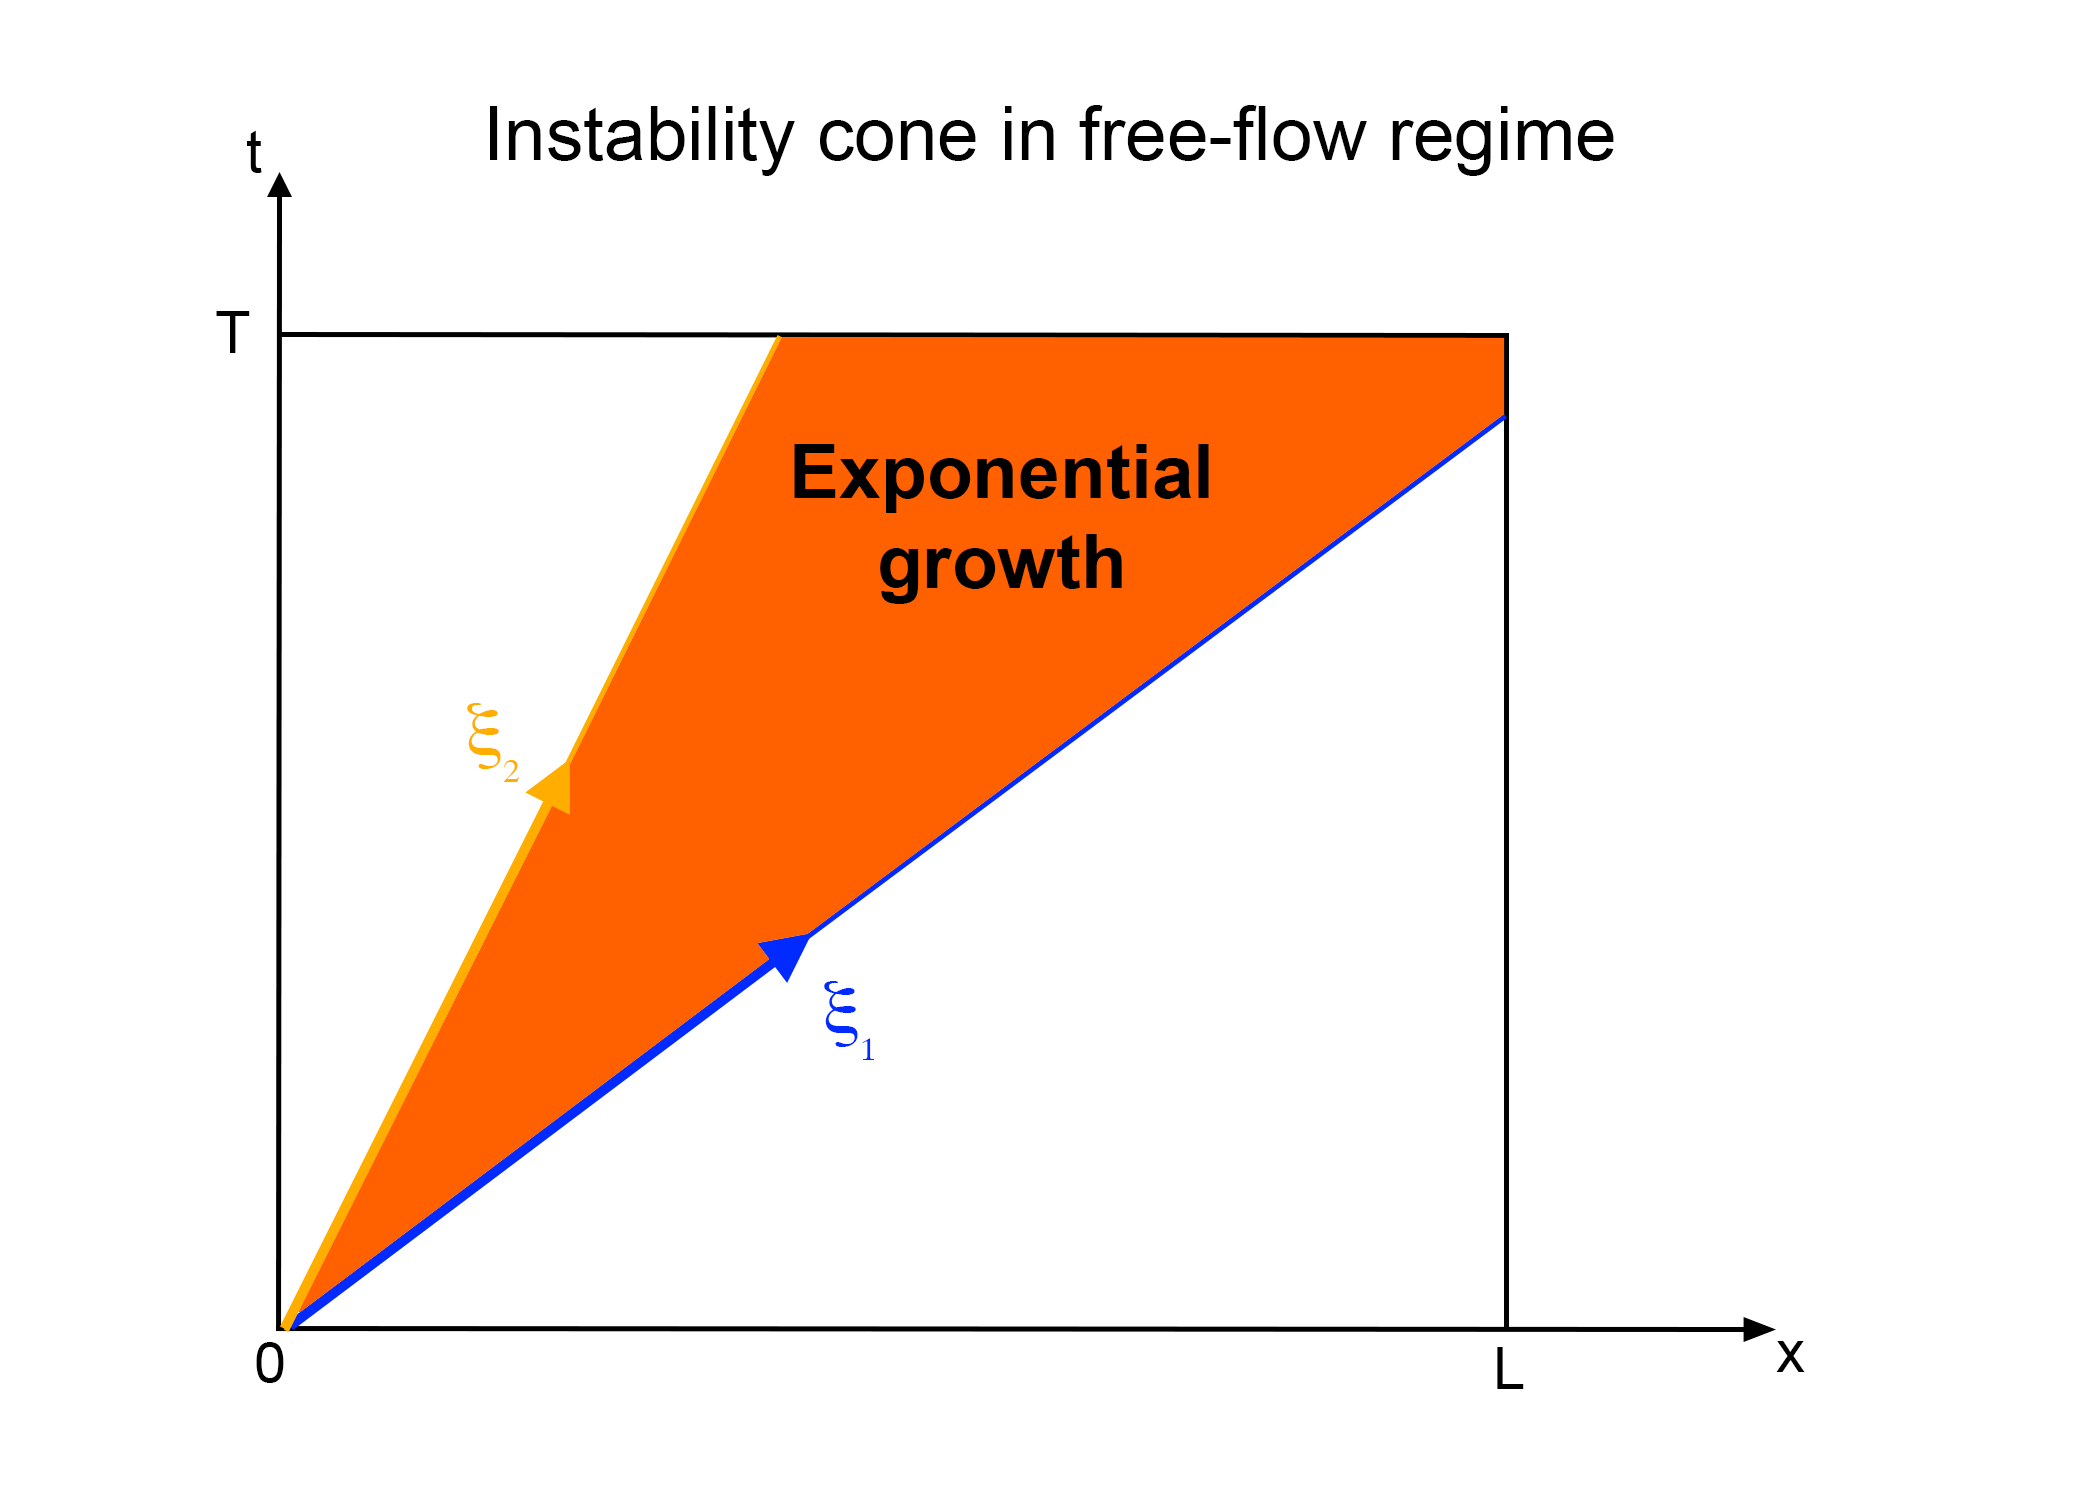
\includegraphics[width=4.5cm]{Exp-growth}
\par\end{centering}
\protect\caption{Illustration of the exponential growth cone appearing in the free-flowing regime for the time domain expressions of $v$ and $q$.\label{Exp-growth}}
\end{figure}

\subsection{Congested regime ($F>1$)}
We now consider the system in the congested regime.

Using \eqref{TFRiemann} we can write 
\begin{equation} \label{vqcongested}
\begin{pmatrix}
\hat{\xi_{1}}(x,s)\\
\hat{\xi_{2}}(x,s)
\end{pmatrix} = \underbrace{
\Phi(x,s) \begin{pmatrix}
1 & 0\\
-\frac{\phi_{21}\left(L,s\right)}{\phi_{22}\left(L,s\right)} & \frac{1}{\phi_{22}\left(L,s\right)}
\end{pmatrix}}_\text{$\Gamma (x,s)$}
\begin{pmatrix}
\hat{\xi_{1}}\left(0,s\right)\\
\hat{\xi_{2}}\left(L,s\right)
\end{pmatrix}.
\end{equation}
with
\begin{subequations}
\begin{align}
\gamma_{11}\left(x,s\right)&=
e^{-\frac{x}{\lambda_{1}}\left(s+\frac{1}{\tau}\right)},\\
\gamma_{12}\left(x,s\right)&=0,\\
\gamma_{21}\left(x,s\right)&=
\frac{\lambda_{1}}{\lambda_{2}}
\frac{\alpha}{s + \alpha}
e^{-\frac{x}{\lambda_{1}} \left( s + \frac{1}{\tau} \right)}
\left(
	1 -
	e^{-\frac{\left(L - x\right)
		}{
		\lambda_{1}\tau\alpha
		}
		\left(s+\alpha\right)
		}
\right)
,\\
\gamma_{22}\left(x,s\right)&=e^{\frac{s\left(L-x\right)}{\lambda_{2}}}.
\end{align}
\end{subequations}

Note that equation \eqref{vqcongested} corresponds to a closed form solution of our initial system, written in spectral form.

For low frequencies ($\left|s\right|\ll\left|\alpha\right|$), 
$\gamma_{21}\left(x,s\right)
\simeq
\frac{\lambda_{1}}{\lambda_{2}}
e^{-\frac{x}{\lambda_{1}} \left( s + \frac{1}{\tau} \right)}
\left(
	1 -
	e^{-\frac{L-x}{\lambda_{1}\tau}}
\right)
$
is the combination of a gain, a distributed delay with propagation speed $\lambda_{1}$, and two distributed gains with characteristic distance $\lambda_{1}\tau$ that cancel out for $x = L$. The resulting bode plot is presented below in Figure \ref{fig:Magn_spatial_diag_congested}.

\subsubsection{Transfer functions for physical variables in congested regime}
In congested regime, the boundary conditions used to control the system are $\hat{\xi}_{1}\left(0,\cdot\right)$ and $\hat{\xi}_{2}\left(L,\cdot\right)$. By linearity of the Laplace transform 
$\hat{\xi_{1}}\left(0,s\right) = 
\frac{
	\rho^{*}\lambda_{2}
}{
	\lambda_{1} - \lambda_{2}
} 
\hat{v}\left(0,s\right)
+
\hat{q}\left(0,s\right)
$.
Therefore, as
$\hat{\xi_{2}}\left(0,s\right) =
\gamma_{21}\left(0,s\right)
\hat{\xi_{1}}\left(0,s\right)
+
\gamma_{22}\left(0,s\right)
\hat{\xi_{2}}\left(L,s\right)$
, we get
$\hat{\xi_{1}}\left(0,s\right) =
\frac{1}{d\left(s\right)}
\hat{q}\left(0,s\right)
+
\frac{n\left(s\right)}{d\left(s\right)}
\hat{v}\left(L,s\right)
$
where
$d\left(s\right) = 1 - \frac{\lambda_{2}}{\lambda_{1}}\gamma_{21}\left(0,s\right)$
and
$n\left(s\right) = \frac{\rho^{*} \lambda_{2}}{\lambda_{1} - \lambda_{2}} \gamma_{22}\left(0,s\right)$. The $\left(v,q\right)$ system has only two degrees of freedom. Therefore we consider that the only inputs to the system are $q\left(0,\cdot\right)$ and $v\left(L,\cdot\right)$. $v\left(0,\cdot\right)$ is then completely determined and can be interpreted as an output of the system. The corresponding transfer equation is
\begin{equation}
\begin{pmatrix}
	\hat{v}\left(x,s\right)
	\\
	\hat{q}\left(x,s\right)
\end{pmatrix}
=
\underset{\Theta\left(x,s\right)}{
\underbrace{
R^{-1}\Gamma\left(x,s\right)
\begin{pmatrix}
	\frac{n\left(s\right)}{d\left(s\right)}
		&
	\frac{1}{d\left(s\right)}	
	\\
	\frac{\rho^{*}\lambda_{1}}{\lambda_{1} - \lambda_{2}}
		&
	0
\end{pmatrix}
}
}
\begin{pmatrix}
	\hat{v}\left(L,s\right)
	\\
	\hat{q}\left(0,s\right)
\end{pmatrix}
\end{equation}
where
\begin{subequations}
\begin{align}
\theta_{11}\left(x,s\right) &=
\frac{
	\alpha 
		e^{
			-\frac{x}{\tau\lambda_{1}}
		}
		e^{
			-\frac{s}{\lambda_{1}}
				\left(
					x - L\frac{\lambda_{1}}{\lambda_{2}}
				\right)	
		}
	+
	s 
		e^{-\frac{s}{\lambda_{2}}\left(x - L\right)}
}{
	s
	+
	\alpha
	e^{-\frac{L}{\tau\lambda_{1}}}
	e^{
	-\frac{sL}{\lambda_{1}}
	\left(
		1 - \frac{\lambda_{1}}{\lambda_{2}}
	\right)
	}
}
,\\
\theta_{12}\left(x,s\right) &=
\frac{
	e^{-\frac{L}{\tau\lambda_{1}}}
	e^{-\frac{s}{\lambda_{2}}
		\left(
			x - L
				\left(1 - 
					\frac{\lambda_{2}}{\lambda_{1}}
				\right)
		\right)
	}
	-
	e^{-\frac{x}{\tau\lambda_{1}}}
	e^{-\frac{sx}{\lambda_{1}}}
}
{
	\rho^{*}\tau
	\left(
		s
		+
		\alpha
		e^{-\frac{L}{\tau\lambda_{1}}}
		e^{
			-\frac{sL}{\lambda_{1}}
			\left(
				1 - \frac{\lambda_{1}}{\lambda_{2}}
			\right)
			}
	\right)
},\\
\theta_{21}\left(x,s\right) &=
\rho^{*}\tau\alpha s
\frac{
	e^{-\frac{s\left(x-L\right)}{\lambda_{2}}}
	-
	e^{-\frac{x}{\tau\lambda_{1}}}
	e^{-\frac{s}{\lambda_{1}}
		\left(
			x - L\frac{\lambda_{1}}{\lambda_{2}}
		\right)
	}
}{
	s
	+
	\alpha
	e^{-\frac{L}{\tau\lambda_{1}}}
	e^{
	-\frac{sL}{\lambda_{1}}
	\left(
		1 - \frac{\lambda_{1}}{\lambda_{2}}
	\right)
	}
},\\
\theta_{22}\left(x,s\right) &=
\frac{
	\alpha
	e^{-\frac{L}{\tau\lambda_{1}}}
	e^{-\frac{s}{\lambda_{2}}
		\left(
			x - L
				\left(
				1 - \frac{\lambda_{2}}{\lambda_{1}}
				\right)
		\right)
	}
	+
	s
	e^{-\frac{x}{\tau\lambda_{1}}}
	e^{-\frac{sx}{\lambda_{1}}}
}{
	s
	+
	\alpha
	e^{-\frac{L}{\tau\lambda_{1}}}
	e^{
	-\frac{sL}{\lambda_{1}}
	\left(
		1 - \frac{\lambda_{1}}{\lambda_{2}}
	\right)
	}
}
.
\end{align}
\end{subequations}

\subsubsection{Low frequency approximation for physical variables in congested regime}
We derive approximate expressions in the frequency domain for the transfer functions above when $\left|s\right|\ll\left|\alpha\right|$:
\begin{subequations}
\begin{align}
\theta_{11}\left(x,s\right) &\simeq
e^{\frac{s\left(L-x\right)}{\lambda_{2}}}
e^{\frac{L-x}{\tau\lambda_{1}}},\\
\theta_{12}\left(x,s\right) &\simeq
\frac{1}{\rho^{*}\tau\alpha}
e^{-\frac{sx}{\lambda_{1}}}
\left(
	1 - e^{\frac{L-x}{\tau\lambda_{1}}}
\right),\\
\theta_{21}\left(x,s\right) &\simeq
s \rho^{*}\tau
e^{\frac{s\left(L-x\right)}{\lambda_{2}}}
e^{\frac{L}{\tau\lambda_{1}}}
\left(
	1 - e^{-\frac{x}{\tau\lambda_{1}}}
\right),\\
\theta_{22}\left(x,s\right) &\simeq
e^{-\frac{sx}{\lambda_{1}}}.
\end{align}
\end{subequations}

With such expressions, interpreting the approximate transfer functions in low frequencies becomes fairly easy.
The transfer function $\theta_{11}$ (resp. $\theta_{12}$) appears as the combination of a distributed delay with propagation speed $-\lambda_{2}$ (resp. $\lambda_{1}$) and a distributed gain (resp. attenuation) with characteristic distance $\lambda_{1}\tau$.
The structure of $\theta_{21}$ is similar to that of $\theta_{11}$ although it features a derivator component.
Once simplified, $\theta_{22}$ corresponds to a distributed delay with propagation speed $\lambda_{1}$.
Hypothetical poles are not active in the range of low frequencies that will be considered in our traffic flow modeling applications.

The eigenvalues of matrix $\Theta(x,s)$ are identical to that of $\Gamma(x,s)$. The latter is lower triangular and its eigen values also have a module bounded by $1$. The congested regime system is therefore also BIBO stable as the $H_{\infty}$ norm of matrix $\Theta(x,s)$ is bounded by $1$.

\subsubsection{Bode plots for congested regime}
We use the same fundamental diagram as in the free-flow case. However the linearization point, $\rho^* = 0.08$ veh/m, corresponds to the congested region of the Greeshields diagram. We show the distributed Bode plots for the Riemann invariants in Figure \ref{fig:Magn_spatial_diag_congested} and for the physical variables in Figure . In that case, $\alpha =$ 0.05 Hz, which does correspond to a reasonable characteristic frequency for traffic modeling applications.

Similarly to the free-flow case, for high frequencies ($w \gg 2 \pi \frac{\lambda_{1} \tau \alpha}{L} = 0.13$ Hz) near zero values appearing with spatial periodicity $\frac{2 \pi}{w} \lambda_{1} \tau \alpha$ almost cancel out $\gamma_{21}$, $\theta_{12}$, and $\theta_{21}$. Such points only appear as irregularities in the Bode plots because the gain is computed on a logarithmic scale.

\begin{figure}
\centering
\begin{tabular}{cc}
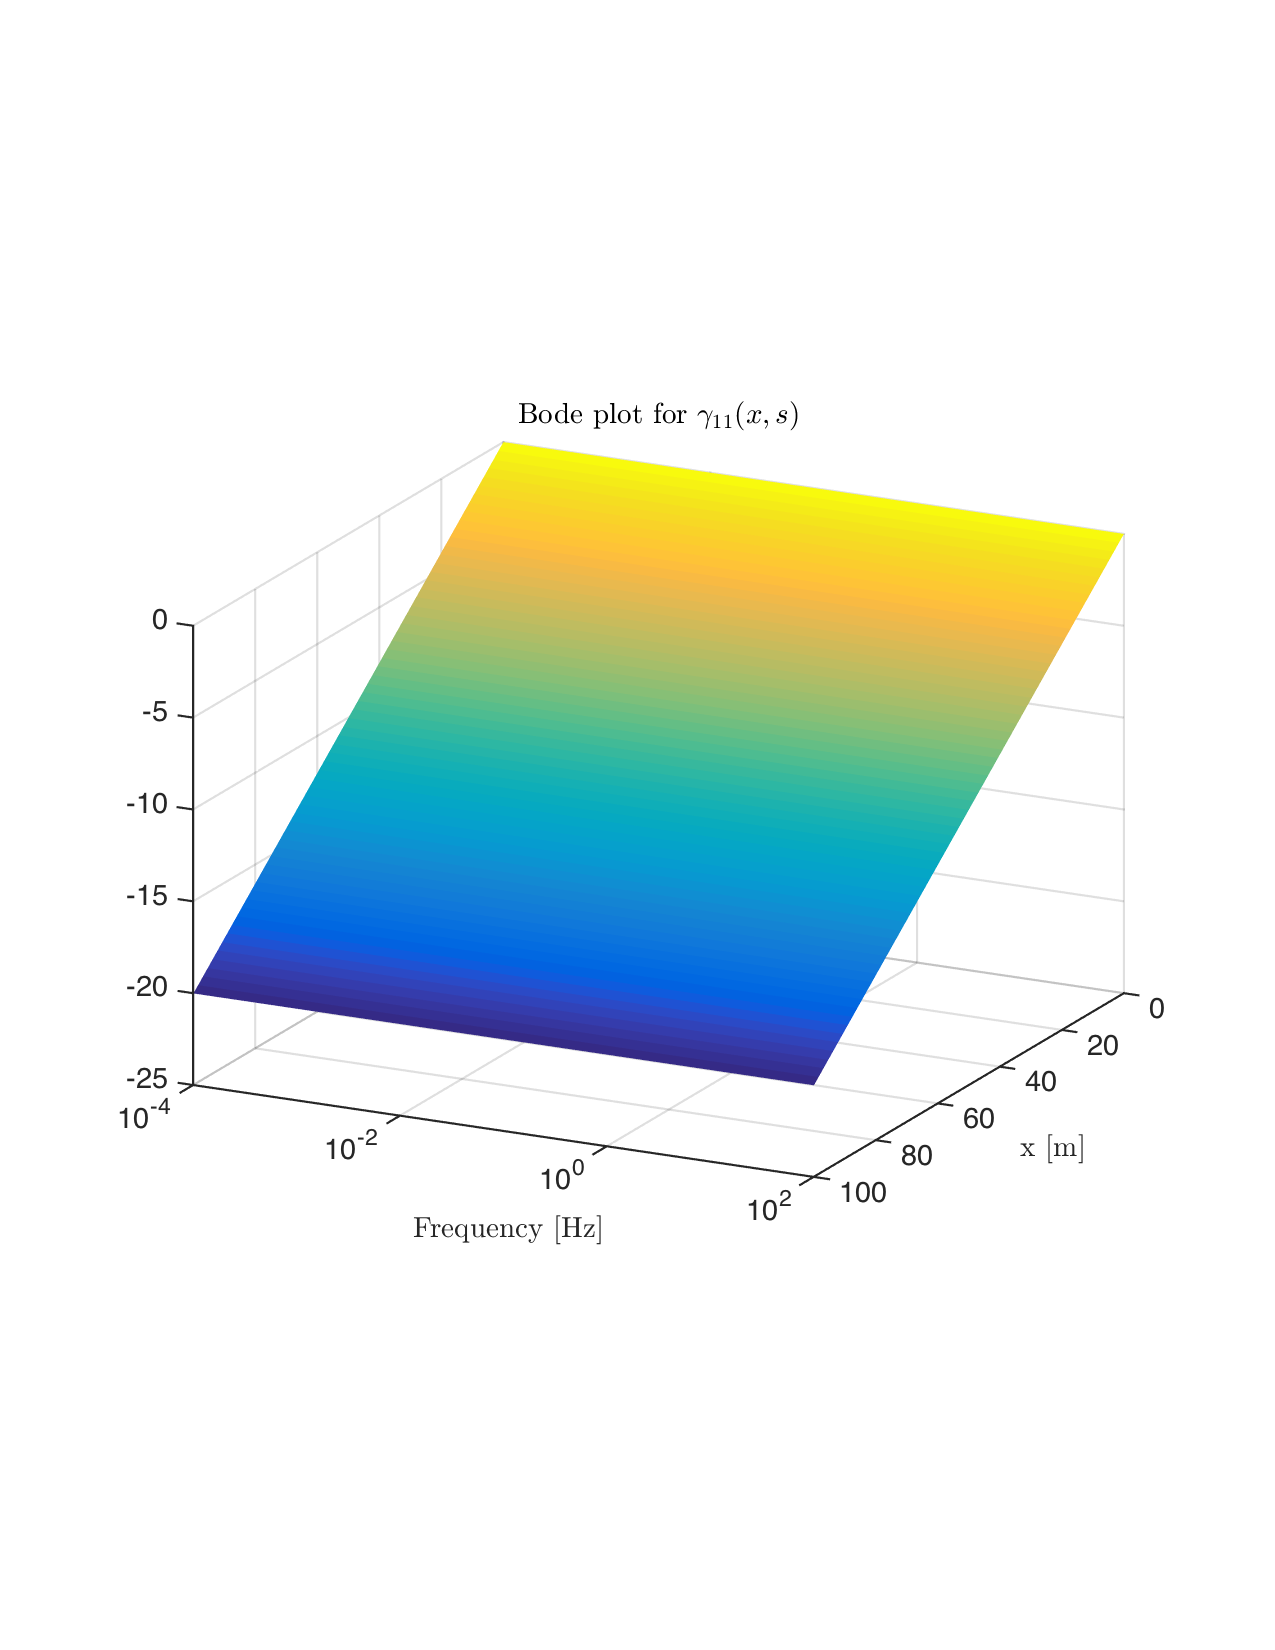
\includegraphics[trim = 0mm 60mm 0mm 60mm, width = 4.2cm]{distr_gamma_11}
&
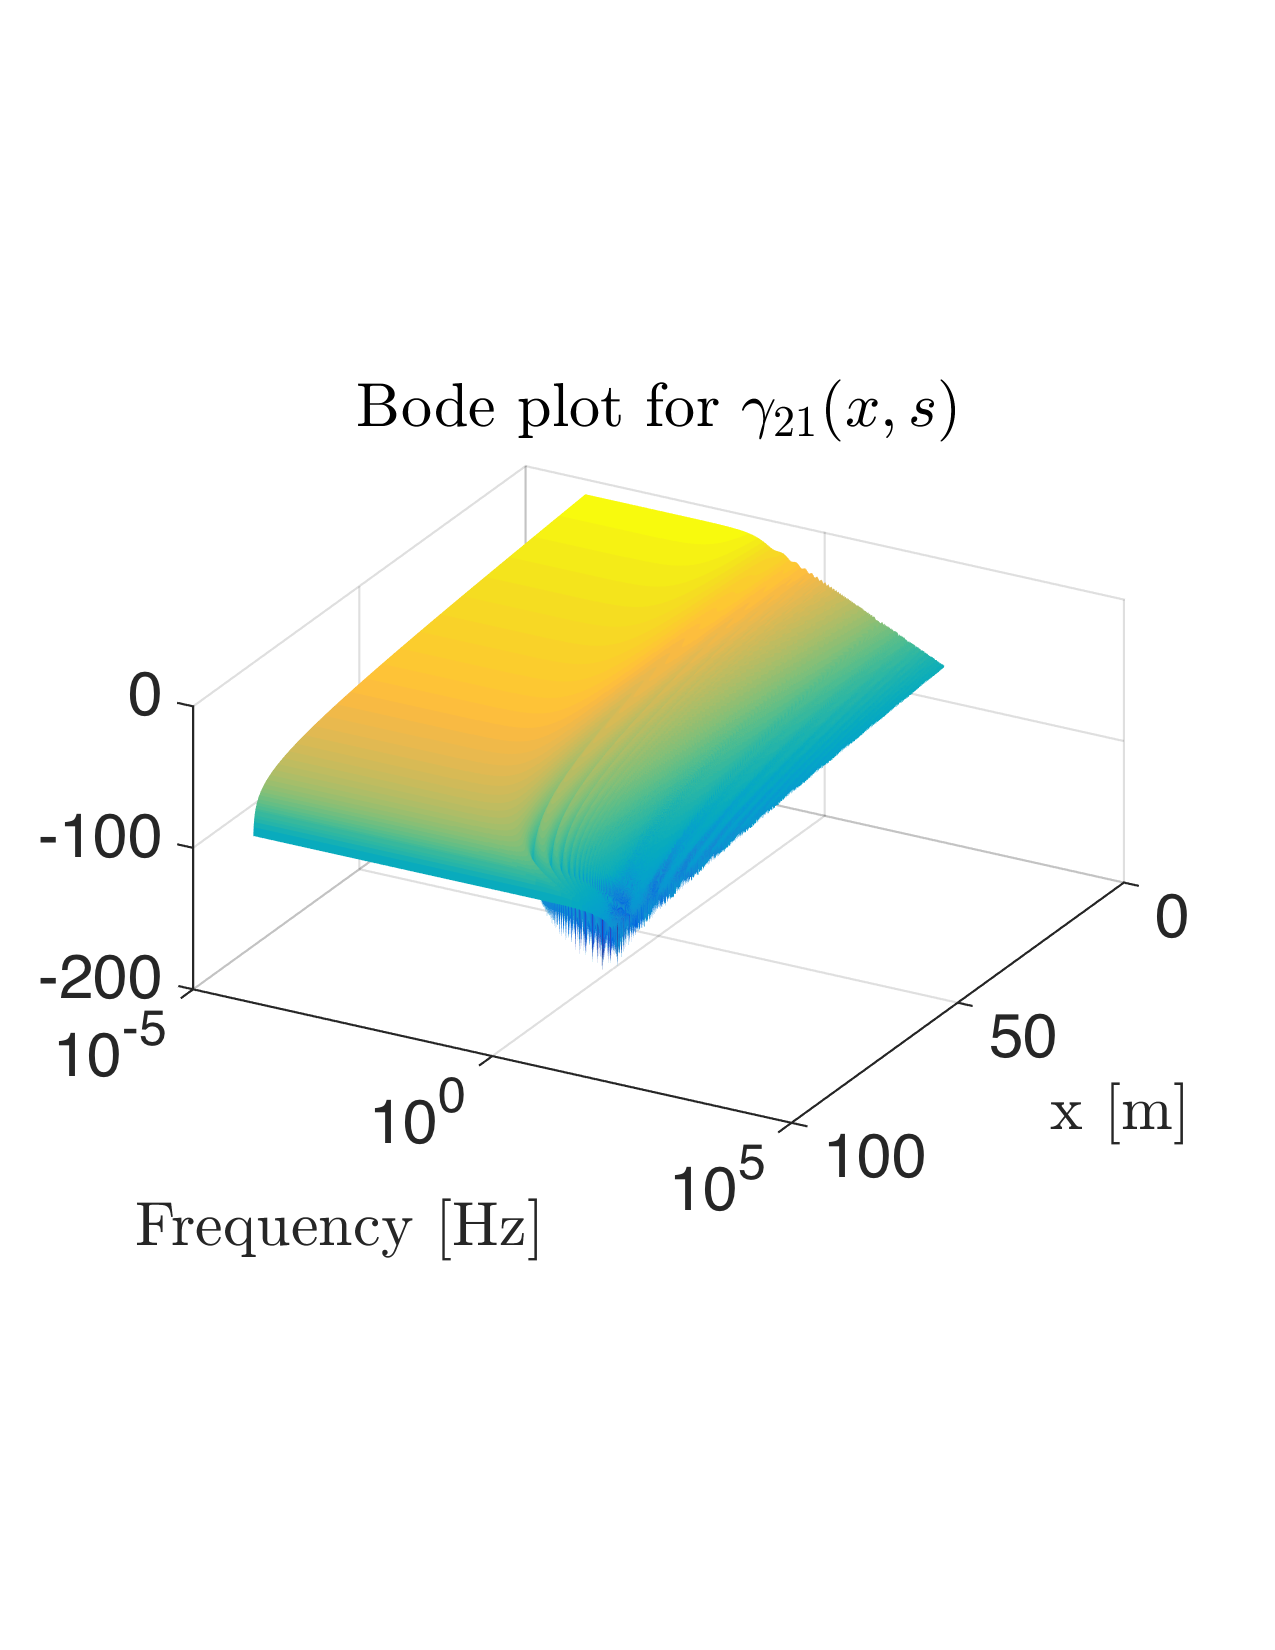
\includegraphics[trim = 0mm 60mm 0mm 60mm, width = 4.2cm]{distr_gamma_21}
\tabularnewline
Bode plot for $\gamma_{11}(x,s)$.
&
Bode plot for $\gamma_{21}(x,s)$.
\tabularnewline
\end{tabular}
\caption{Spatial magnitude Bode plots for Riemann invariants in congested regime ($\left|\alpha\right| = $ 0.05 Hz)\label{fig:Magn_spatial_diag_congested}}
\end{figure}

\begin{figure}
\centering
\begin{tabular}{cc}
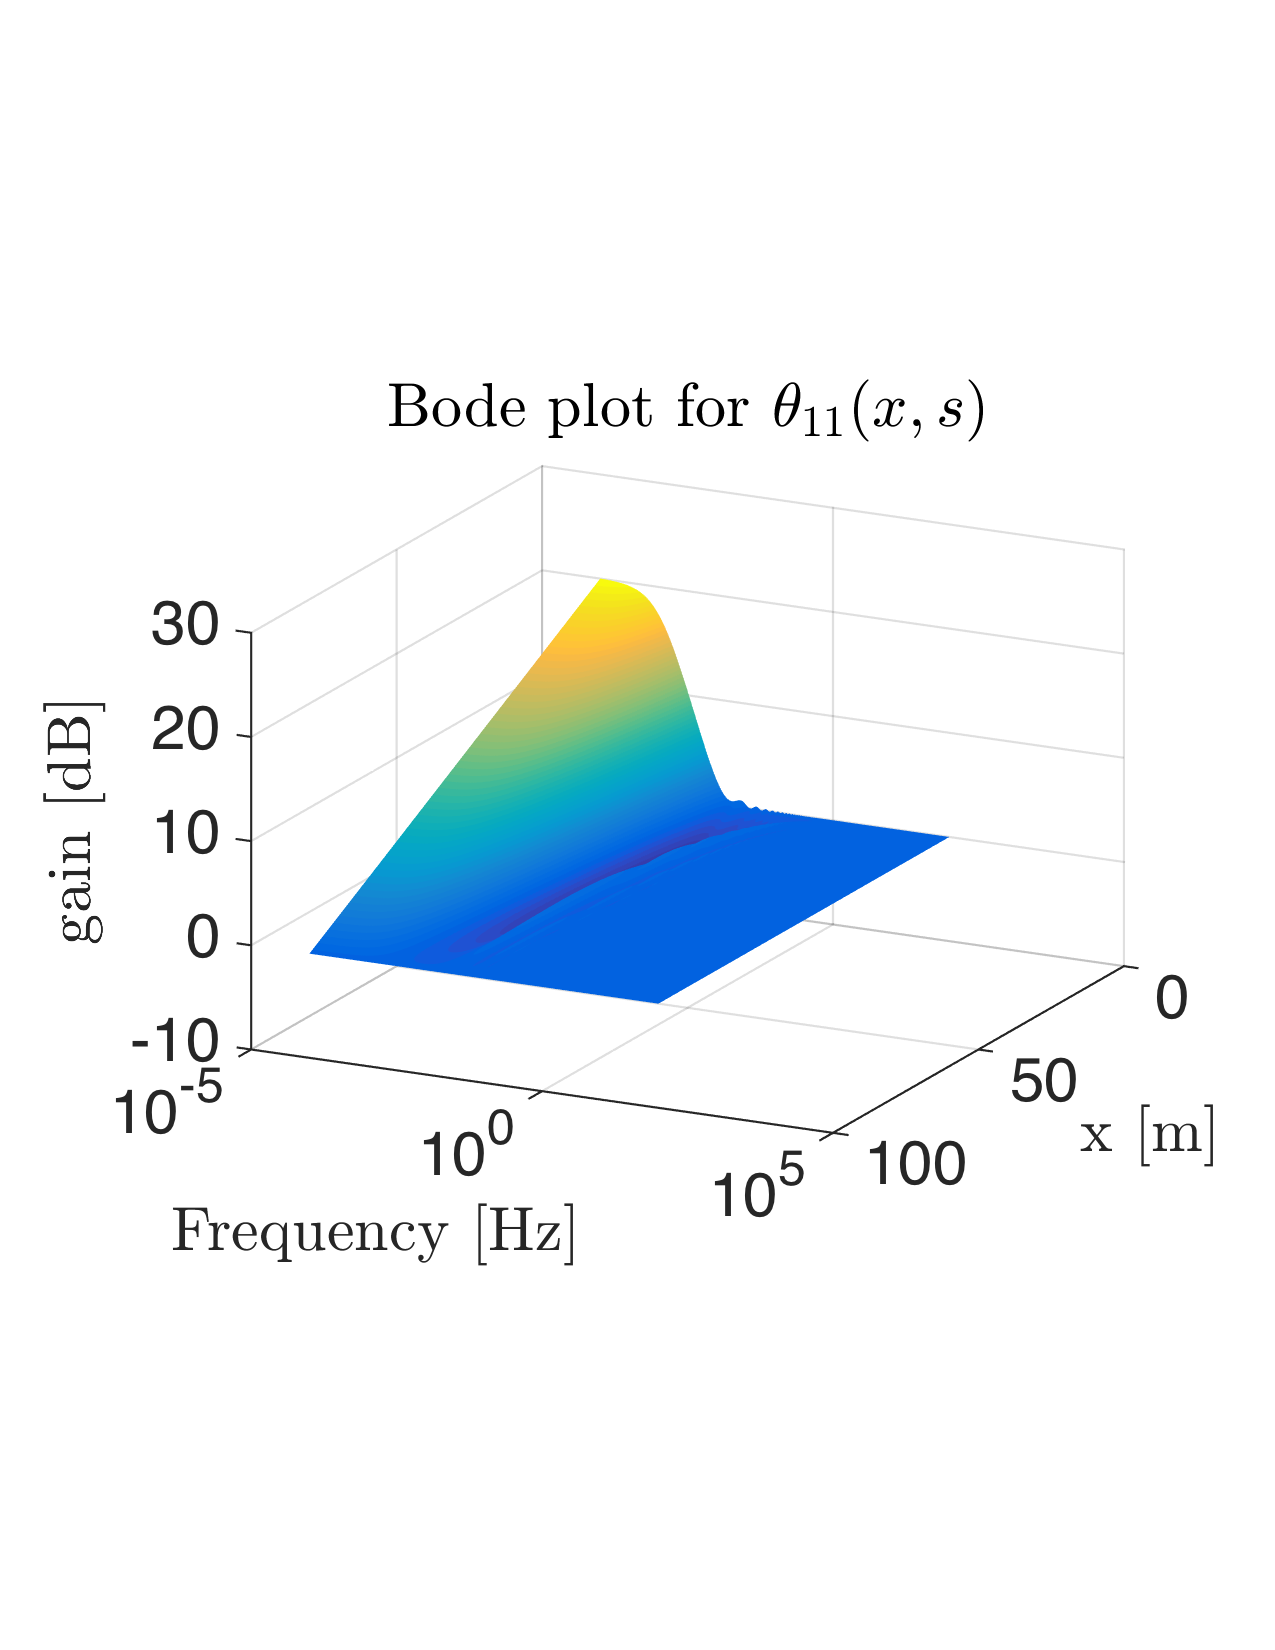
\includegraphics[trim = 0mm 60mm 0mm 60mm, width = 4.2cm]{distr_theta_11}
&
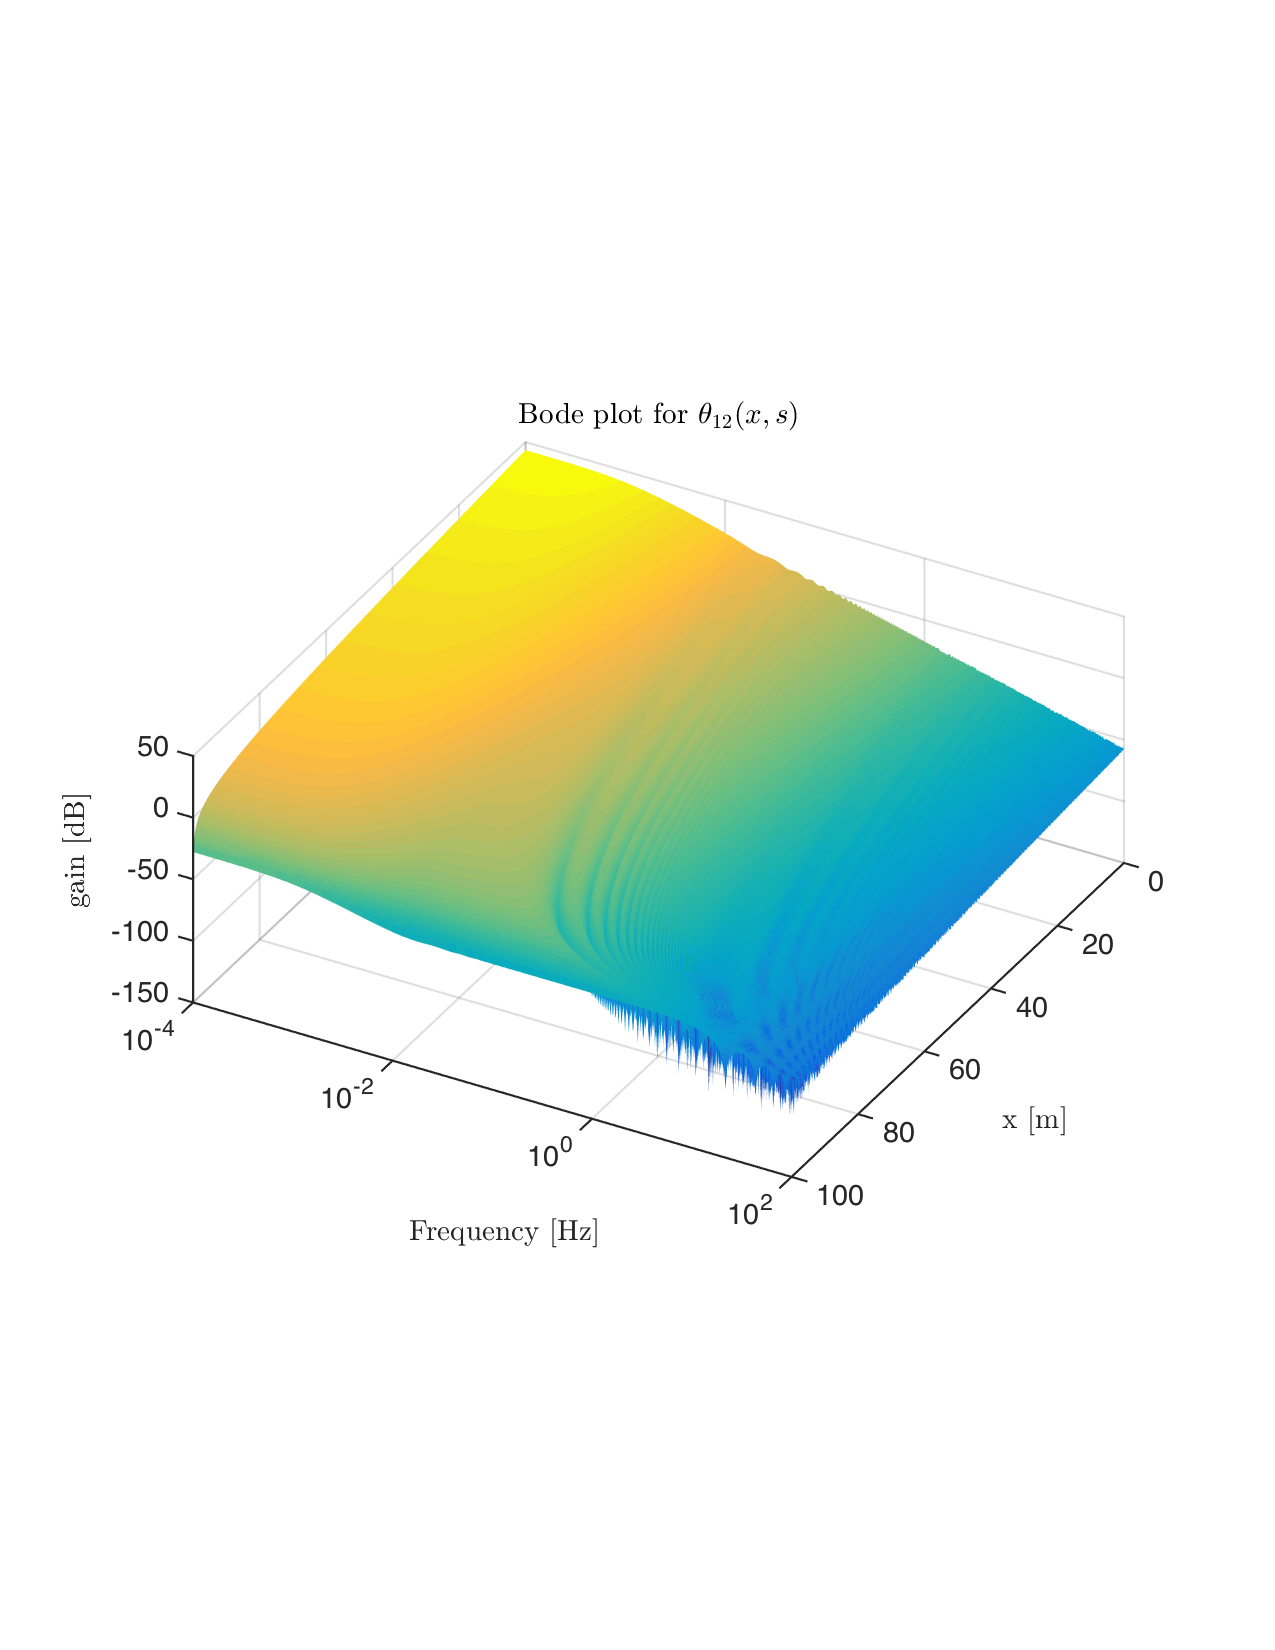
\includegraphics[trim = 0mm 60mm 0mm 60mm, width = 4.2cm]{distr_theta_12}
\tabularnewline
Bode plot for $\theta_{11}(x,s)$.
&
Bode plot for $\theta_{12}(x,s)$.
\tabularnewline
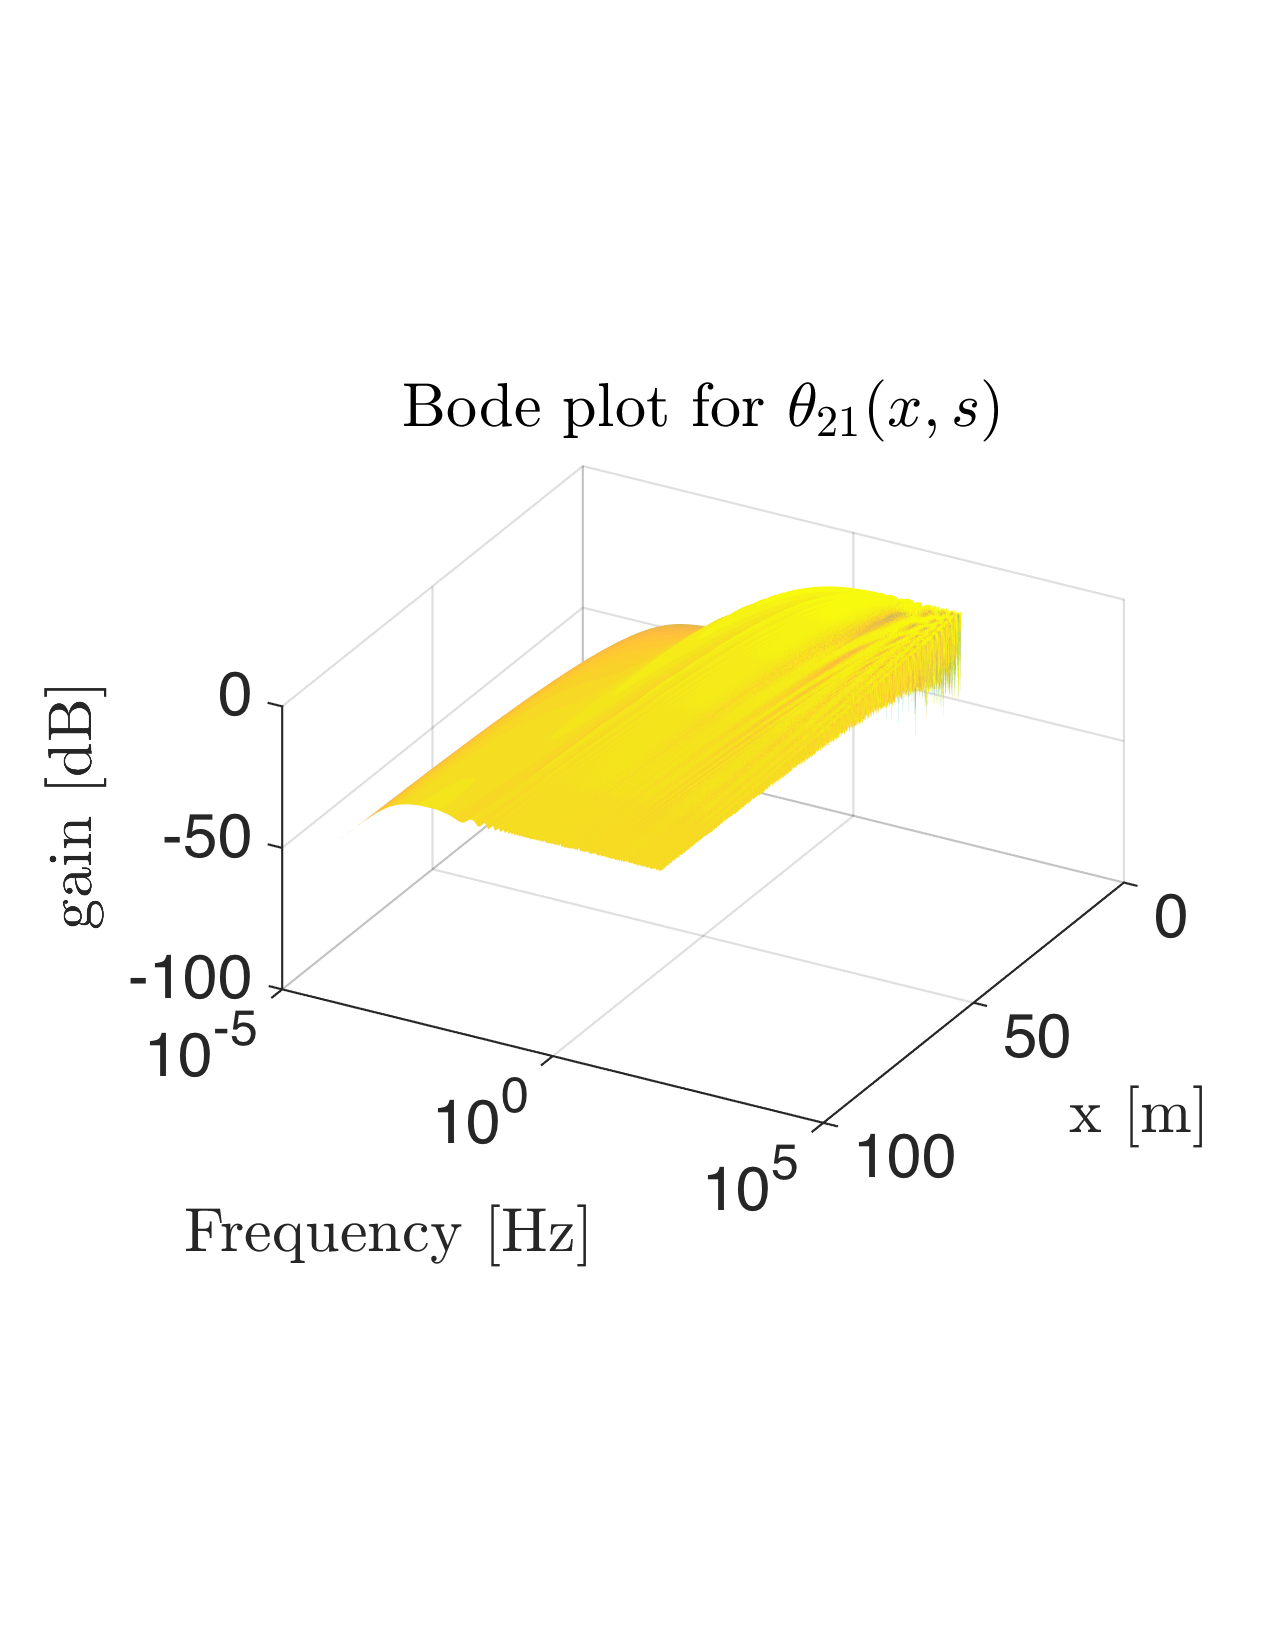
\includegraphics[trim = 0mm 60mm 0mm 60mm, width = 4.2cm]{distr_theta_21}
&
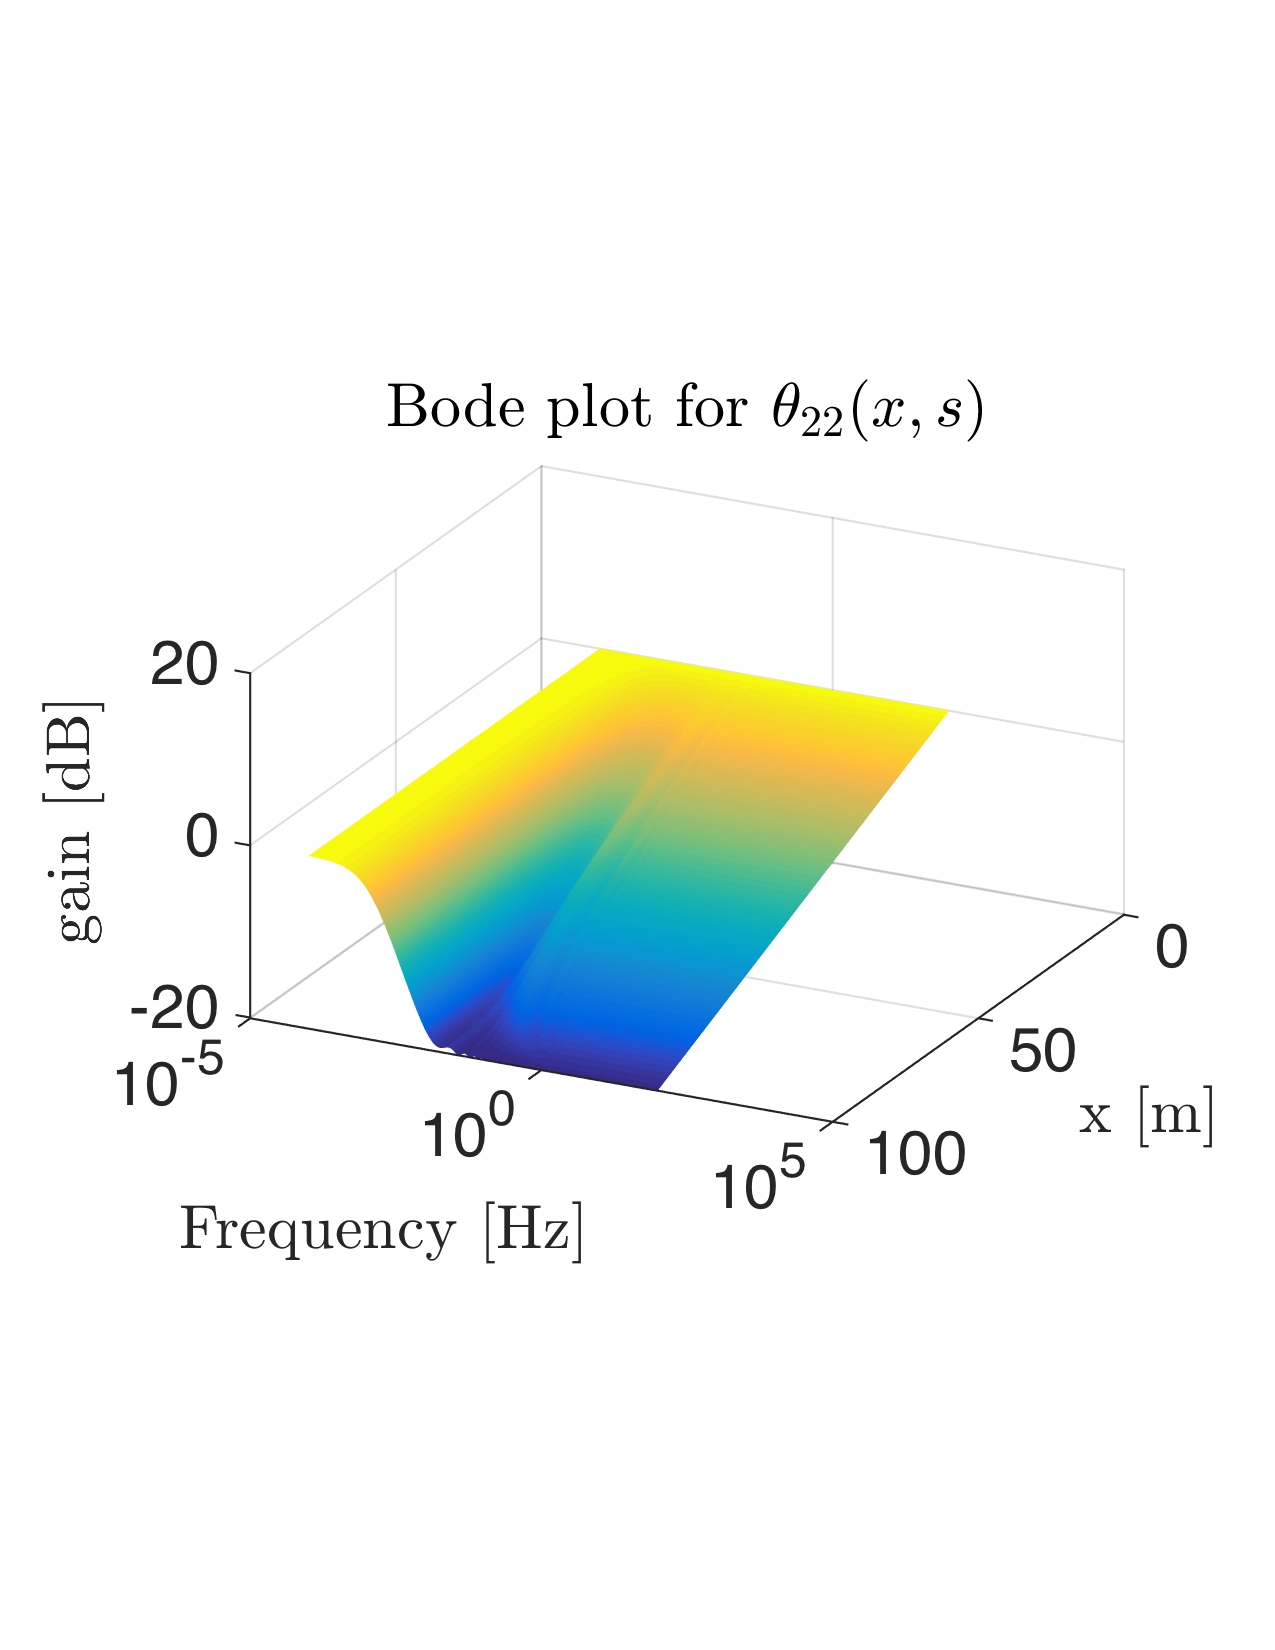
\includegraphics[trim = 0mm 60mm 0mm 60mm, width = 4.2cm]{distr_theta_22}
\tabularnewline
Bode plot for $\theta_{21}(x,s)$.
&
Bode plot for $\theta_{22}(x,s)$.
\tabularnewline
\end{tabular}
\caption{Spatial magnitude Bode plots for physical variables in congested regime ($\left|\alpha\right| = $ 0.05 Hz)\label{fig:Magn_spatial_physx_congested}}
\end{figure}

\subsubsection{Poles and BIBO stability of the system}
In order to practically assess the presence of poles, numerical search for roots of the denominator of the transfer functions has been conducted thanks to standard equation solvers. Once more $-\alpha$ is a solution and another one was found at $s=-0.0018$. They are both negative reals and therefore cannot make the system unstable. Although the solvers could have detected poles with a non zero imaginary part, none has been found. Holistic search for other poles should be conducted but is out of the scope of this article.

\subsection{Findings and conclusion from the theoretical study}
The numerical experiments above have validated the accuracy of the linearized model and highlighted several of its core properties.

The TFN delineates two regimes: congested for $F > 1$ and free-flowing for $F < 1$. This classification, and the resulting stability result legitimize the use of linearization about a nominal point in the stable region.

The assessment of convective instability in the free flow regime is of course applicable to this specific model (other models such as \cite{Jamitons-multi-valued-fund} might lead to other conclusions, and all need to be checked against experimental data). Here, exponential growth of the linearization error only occurs in a conic region of the  $\left[0,T\right] \times \left[0,L\right]$ domain where convective instability travels along the characteristics.

The absolute value of the term $\alpha = -\dfrac{\lambda_2}{\tau(\lambda_1 - \lambda_2)}$ is a characteristic frequency of the system. It delineates the low frequency domain in which approximate expressions help decompose the transfer functions in simple gain and delay components. In the spectral domain, $\lambda_{1}$ and $\lambda_{2}$ appear as information propagation speeds in distributed delay elements while  $\tau\lambda_{1}$ acts as the characteristic distance of distributed gain components.


\section{Numerical validation}

In this section we demonstrate the ability of the linearized ARZ equations to model the various nonlinear dynamics around a nominal operation point and compare the prediction of the model with actual flow and velocity data gathered from the well-known NGSIM data set.


\subsection{Data source: NGSIM trajectories}

We use the NSGIM trajectory data set for a section of the US-101 highway. The set gathers trajectories of vehicles sampled with a 10 Hz frequency thanks to high precision cameras. The data is pre-processed so as to take only cars into account; 45 minutes are recorded on a 650-meter long section with five lanes. The lanes are taken into account when computing the lineic density of vehicles $\rho$.
A map of the time evolution of speed along the section is given in Figure \ref{fig:NGSIM-trajectories}.
Only a subset of the spatial domain is used due to the presence of ramps, which breaks the homogeneity of the freeway. The viable domain is 200 meters long.

\begin{figure}
\centering
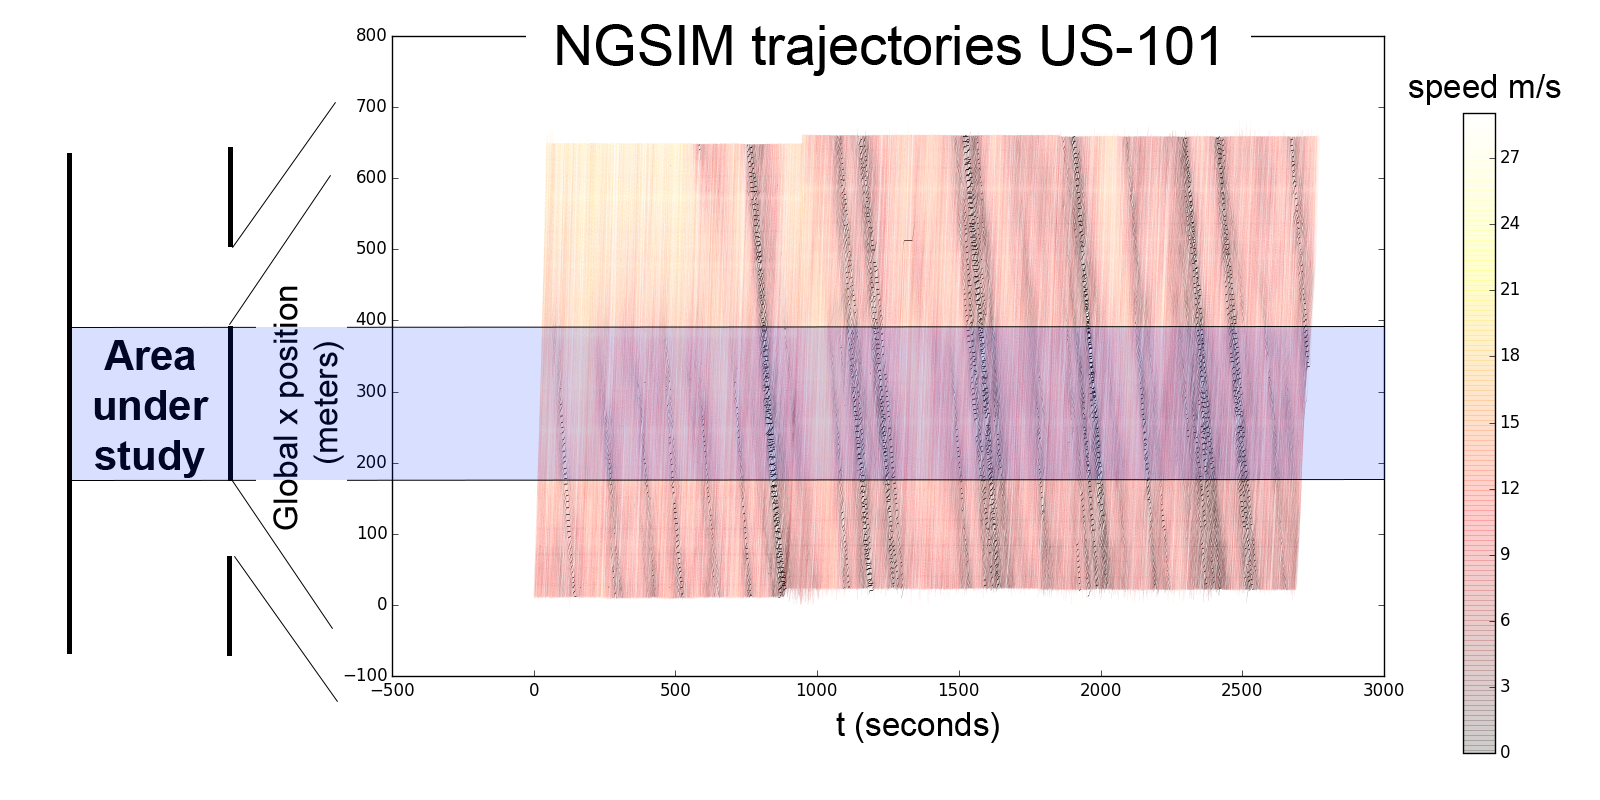
\includegraphics[width=8cm]{US-101_all_traj_low_res_mod}
\protect\caption{NGSIM trajectories. Color represents the measured speed of each
car in m/s.}
\label{fig:NGSIM-trajectories}
\end{figure}



\subsection{Reconstructing $(v,q)$ maps from NGSIM trajectories}

The NGSIM data set does not directly provide the values $v(t,x)$
and $q(t,x)$ in the resolution domain $\left[0,T\right]\times\left[0,L\right]$. To obtain macroscopic quantities out of the microscopic measurements, we follow the approach devised in \cite{edie1963discussion} and divide the space-time grid into cells $\left(\left[i\Delta t,\, \left(i+1\right)\Delta t\right]\times\left[j\Delta x, \, (j+1)\Delta x\right]\right)_{i\in\left\{ 1\ldots n_{t}\right\} ,j\in\left\{ 1\ldots n_{x}\right\} }$, where $n_t$ and $n_x$ are the number of cells in time and space, respectively. We denote each cell as $\bin_{i,j}$. This operation consists of gathering corresponding data points into cells, then estimating the quantities of interest in each cell, it was for example used in \cite{Piccoli201532}.

Within each cell, a specific number of traces, or footprints of a vehicle along its trajectory, are available, and $\rho$, $v$, and $q$ are assumed to be constant. We present several formulae to map a set of traces to speed, flow, and density over the space-time grid. 

\textbf{Binning formula for $v$}: Since the speed is assumed to be constant in each cell, a straightforward estimate for the speed is the empirical average. The estimator for $v$ in $\bin_{i,j}$ is

\begin{equation}
\widehat{v}_{i,j}=\mean_{\trc \in \bin_{i,j}}(v(\trc)).
\end{equation}

\textbf{Binning formula for $\rho$}: By definition, the density of $\bin_{i,j}$ is  
\begin{equation}
\rho_{i,j}=
\frac{\iint_{\left(t,x\right)\in [i\Delta t, \,(i+1)\Delta t] \times [j\Delta x,\,(j+1)\Delta x]}\rho(x,t) \text{d}x \text{d}t}
{n_{\lns}\Delta x\Delta t}
.
\end{equation}

The position of each vehicle is recorded every 0.1 second. For each cell we count the number of traces and normalize it by the sampling rate. The contribution of a given vehicle to the density of a cell is proportional to the number of traces it has left in the cell. If the speed is assumed to be locally constant, this contribution is proportional to the time this vehicle spends in the cell and is consistent with the conservation of the total number of vehicles across all cells. Then we have the density estimator


\begin{equation}
\widehat{\rho}_{i,j}=
\frac{\card ( \{ \trc \mid \trc \in \bin \})}
{n_{\lns} \Delta x \Delta t \: \text{sampling rate}},
\end{equation}
where $\card (\cdot)$ gives the number of elements in a set, i.e., its cardinal. 

\textbf{Binning formula for $q$}: By definition, $q=\rho v$, so a logical first estimate for $q$ in $\bin_{i,j}$ is 
\begin{equation}
\widehat{q}_{i,j}=\widehat{v}_{i,j}\widehat{\rho}_{i,j}.
\end{equation}

We can also approximate the flux through $\bin_{i,j}$ with a simple counting method. If a vehicle crosses spatial coordinate $\left(j+1\right)\Delta x$ between times $i\Delta t$ and $\left(i+1\right)\Delta t$, then it leaves a trace in both $\bin_{i,j}$ and $\bin_{i,j+1}$. Counting these vehicles and normalizing by the duration $\Delta t$ gives the estimator

{\footnotesize
\begin{align}
&\widehat{q}_{i,j}^{\cnt}= \notag \\
&\frac{\card\left(\left\{ \text{id} \left(\trc\right)\mid \trc \in \bin_{i,j}\right\} \cap\left\{ \text{id}\left( \trc \right)\mid \trc\in \bin_{i,j+1}\right\} \right)}{n_{\lns}\Delta t},
\end{align}
}

where id$(\cdot)$ gives the identification number of a vehicle.



\subsubsection{Choosing the number of bins}

As the estimation formulae above rely on averaging, having a comfortable
number of points in each bin provides more stable estimates. It is worth mentioning that usual central limit theorem based reasoning for convergence of such estimates is flawed as several samples may correspond to the same vehicle or interacting vehicles, violating the independence assumption of the theorem. Proving the convergence of the estimates above lies beyond the scope of this article. As a rule of thumb we choose a discretization that guarantees that most bins will host more than $100$ traces. This is achieved with a $80\times80$ grid where the $10^{\text{th}}$ percentile of the number of traces in a given bin is $170$. Such a grid also yields a $10^{\text{th}}$ percentile of $56$ distinct vehicles per bin. The histograms of number of traces and vehicle per cell are given in Figure \ref{fig:Grid control}.

\begin{figure}
\centering
\begin{tabular}{cc}
\includegraphics[width=6cm]{\string"traces_80_80\string".png} 
\tabularnewline
Histogram of number of traces per cell. 
\tabularnewline
\includegraphics[width=6cm]
{\string"ids_80_80\string".png}
\tabularnewline
Histogram of number of distinct vehicles per cell.
\end{tabular}
\caption{Experimental justification for a $80\times 80$ cell based discretization
grid for the NGSIM data.}
\label{fig:Grid control}
\end{figure}

While our goal here is not to present theoretical proofs of the convergence of the binned estimators for $\left(v,\rho,q\right)$, it is nonetheless possible to check that the procedure is coherent. Two estimators are provided for $q$ that use radically
different techniques: the first relies on the average measured speed and the number of traces in a bin, while the other relies on counting vehicles transiting from a cell to another. Figure \ref{fig:Sanity-check} show that the scatter plot of $\widehat{q}_{i,j}^{\cnt}$ plotted against $\widehat{q}_{i,j}$ coincides nicely with the line $y=x$, validating the overall binning and estimation procedure above.

\begin{figure}
\centering
\includegraphics[width=6cm]{\string"80_80_q_q_count\string".png}
\protect\caption{Sanity check for the estimation procedure. $\widehat{q}_{i,j}^{\text{count}}$
is plotted against $\widehat{q}_{i,j}$ across the grid of bins.
\label{fig:Sanity-check}}
\end{figure}



\subsection{Estimated values for $\left(v,q\right)$} 

To check how well the linearized ARZ model fits an actual dataset, we chose a bounded domain and compare the theoretical solution given by the second-order model and the observed data. Again we focus on the variables $v$ and $q$. Using the estimation procedure above, we compute fundamental diagrams from which we estimate the eigenvalues $\lambda_{1}$ and $\lambda_{2}$.
To calibrate the relaxation time $\tau$, we analyze the errors of predicted values of $v$ and $q$ for various $\tau$. The resulting maps of both the predicted and observed values highlight phenomena that the linearized model can and cannot account for. 

\textbf{Maps.} The estimates $\widehat{v}_{i,j}$, $\widehat{\rho}_{i,j}$, $\widehat{q}_{i,j}$, and $\widehat{q}_{i,j}^{\text{count}}$ are plotted on the discretized grid in Figure \ref{fig:Data-versus-predicted.}. Note that $\widehat{q}$ and $\widehat{q}^{\text{count}}$ give extremely similar results, so we may use $\widehat{q}^{\text{count}}$ from this point on. Damped oscillations and smoothly decaying values along characteristic lines are the main characteristic the practical implementation of the model should feature.

\textbf{Fundamental diagrams.} From the estimated values we can easily compute the fundamental diagram. We use the fundamental diagrams to calibrate the model parameters. Though the dataset used is dense, it covers only a small region of time and space. Thus, its small size is a potential flaw in our model parameter calibration as it is certain that
our measurements are highly correlated. This seems
to be confirmed by the fact that the fundamental diagrams below correspond only to the congested regime. \

\textbf{Calibration of $\lambda_{1}$ and $\lambda_{2}$, linearization point.} In Section \ref{ARZSection}, we found that $\lambda_{1}$ is exactly $v^*$ and $\lambda_{2}$ is the slope of the fundamental diagram at $v^*$. Thus to calibrate the eigenvalues we must find the linearization point. We estimate the linearization point using the Ordinary Least Squares method. Note the dataset used corresponds only to the congested regime and the fundamental diagram is almost affine. The estimator, $\widehat{\lambda}_1=\widehat{v}^*$ is chosen as the empirical mean of $\widehat{v}_{i,j}$. To estimate $\lambda_{2}$, we fit a linear model $\widehat{q}^{\text{count}}=b_{1}\widehat{\rho}+b_{0}+\varepsilon$, where $\varepsilon$
represents the noise in the model that would ideally be centered,
homoschedastic, and uncorrelated but is not practically. Then $\widehat{\lambda}_{2}=\widehat{b}_{1}$ and we take $\widehat{q}^*$ as the empirical average of $\widehat{q}^{\cnt}$. The ratio of $\widehat{q}^*$ and $\widehat{v}^*$ gives the estimate $\widehat{\rho}^*$.
Provided each estimator is convergent, the continuity of the functional
$\left(x,y\right)\rightarrow\frac{x}{y}$ on its domain guarantees the convergence of $\widehat{\rho}^*$. The empirical results are presented in Figure \ref{fig:Calibration-of-eigen-values}. The determination coefficient is poor but can be improved by filtering out outliers and gathering more data. Future work should include improving the quality of the estimation. Significance tests for the coefficients of the linear model are not presented. The assumptions they rely on about
the linear dependency between $\widehat{q}$ and $\widehat{v}$ are clearly
not respected here as the noise is auto-correlated. Further work should also turn this rather heuristic method for estimating parameters
into a fully justified statistical procedure. Note that the goal of the present article is to provide a new model and corresponding spectral analysis, which we want to illustrate with state of the art data. Thus, development of statistical methods to handle this data is out of the scope of the present investigation.

\begin{figure}
\centering
\includegraphics[width=6cm]{\string"Fundamental_diagram_fitting_n_80\string".png}
\protect\caption{Calibration of $\lambda_{1}$ and $\lambda_{2}$. The circle denotes the linearization point. The affine model used to estimate $\lambda_{2}$ and the linearization point is also plotted. The estimates are: $\widehat{\lambda}_{1}=8.96$ m/s, $\widehat{\lambda}_{2}=-4.37$ m/s, $\widehat{\rho}^{*}=0.049$ veh/m, $\widehat{v}^{*}=8.96$ m/s, $\widehat{q}^{*}=0.44$ veh/s, with $r^{2}=0.48$. The characteristic frequency of the system is $\widehat{\alpha} = 8.37\times10^{-3}$ Hz. Its order of magnitude does correspond to practical traffic flow modeling.}
\label{fig:Calibration-of-eigen-values}
\end{figure}

\subsection{Verification of the spectral form}
In this section we demonstrate the performance of the spectral form as a prediction tool using the time domain responses derived from the transfer functions and FFT. Since we are working with a linearized system, we can decompose boundary conditions then add predicted values inside the domain $\left[0,T\right]\times\left[0,L\right]$. Fourier decomposition of boundary conditions is here extremely accurate as the median relative errors for the interpolation of the values of $\xi_{1}\left(x=0, \cdot \right)$ and $\xi_{2}\left(x=L, \cdot \right)$ are respectively $2\%$ and $3\%$.

\textbf{Simulated maps.} Since the spectral form presents information in the diagonalized basis, we need a conversion before we can compare the simulated results to the values estimated from the dataset.  
To make a comparison in the diagonalized basis, we first compute the estimated deviations from the equilibrium $\widehat{\widetilde{v}}_{i,j}=\widehat{v}_{i,j}-\widehat{v}^{*}$ and $\widehat{\widetilde{q}}_{i,j}=\widehat{q}_{i,j}-\widehat{q}^{*}$. Then the estimates for $\xi_{1}$ and $\xi_{2}$ are given by $\widehat{\xi}_{1_{i,j}}=\frac{\widehat{\rho}^{*}\widehat{\lambda}_{2}}{\widehat{\lambda}_{1}-\widehat{\lambda}_{2}}\widehat{\widetilde{v}}_{i,j}+\widehat{\widetilde{q}}_{i,j}$ and
$\widehat{\xi}_{2_{i,j}}=\frac{\widehat{\rho}^{*}\widehat{\lambda}_{1}}{\widehat{\lambda}_{1}-\widehat{\lambda}_{2}}\widehat{\widetilde{v}}_{i,j}$. To compare the physical variables, we compute the velocity and flow predictions by inverting \eqref{eq:Riemannzeta}: $\widetilde{q}=\xi_{1}-\frac{\lambda_{1}}{\lambda_{2}}\xi_{2}$,
$\widetilde{v}=\frac{\lambda_{1}-\lambda_{2}}{\rho^{*}\lambda_{1}}\xi_{2}$.

Figure \ref{fig:Data-versus-predicted.} shows important qualitative properties of the model. As expected, the model generally predicts with very good accuracy the decay of all quantities along their characteristic lines, a realistic feature that cannot be paralleled by first-order models. The general quality of the fit is rather good with most of the error on $v$ and $q$ in a $20\%$ range of the data's amplitude between minimum and maximum values. Furthermore the linearized second-order model manages to capture oscillations observed on the boundary and account for their decay accurately. 

\textbf{Error analysis}
Examining the empirical distributions of errors and relative errors for speed and flow in Figure \ref{fig:q-error.} reveals important facts about the accuracy of the linearization procedure. In particular, although most of the flow and speed finally predicted in each bin is closed to the data (the relative error is mostly below $20\%$), the errors distributions are skewed negatively and have a negative median (in particular those of $v$). This means the procedure has a tendency to under-estimate speed and flow as we can see negative bias in the predictions. The calibration of eigen values is core to the whole analysis and improving it could alleviate this phenomenon.

\begin{figure}
\centering
\begin{tabular}{c}
\includegraphics[width=8cm]{\string"q_error_80_best_tau\string".png}\tabularnewline
\includegraphics[width=8cm]
{\string"v_error_80_best_tau\string".png}
\end{tabular}
\protect\caption{Distribution of prediction errors (each sample is the error corresponding to a single discretization cell).\label{fig:q-error.}}
\end{figure}


\textbf{Calibration of $\tau$\label{sub:Calibration-of-tau}} For each $\tau$ we compute the \textit{mean absolute error} (MAE), or the average difference in absolute value between simulated and predicted values for each discretization cell. Since the quantities $v$ and $q$ are not physically homogeneous, it is not sensible to aggregate the errors over these quantities. However, $\xi_{1}$
and $\xi_{2}$ are both expressed in veh/s. Summing their MAE gives a reliable uni-dimensional index of the quality of the fit with respect
to $\tau$. This quantity is computed for different values of $\tau$
ranging from 5 to 80 seconds. The value offering the best fit
is $\tau^{*}=39.18$ s.

\begin{figure}
\centering
\begin{tabular}{c}
\includegraphics[width=9cm]{\string"vq_map_n_80_best_tau\string".png}\tabularnewline
\includegraphics[width=9cm]
{\string"xi_map_n_80_best_tau\string".png}
\end{tabular}
\protect\caption{Data versus predicted. Top Figure: $\left(v,q\right)$ domain, top row is $v$, bottom row is $q$. Bottom: $\left(\xi_{1},\xi_{2}\right)$
domain, top row is $\xi_{1}$, bottom row is $\xi_{2}$. First column: data. Middle column: predictions. Third column: error (difference between prediction and data).\label{fig:Data-versus-predicted.}}
\end{figure}

\begin{figure}
\centering
\begin{tabular}{cc}
\includegraphics[width=6cm]
{\string"q_v_error_80\string".png} 
\tabularnewline
MAE over $q$ and $v$
\tabularnewline
\includegraphics[width=6cm]{\string"xi_1_xi_2_error_80\string".png}
\tabularnewline
MAE over $\xi_{1}$ and $\xi_{2}$ and sum of MAEs.
\end{tabular}
\protect\caption{Calibration of $\tau$, one minimizes the sum of MAE over $\xi_{1}$
and $\xi_{2}$.}
\end{figure}


\subsection{Findings and conclusion from the numerical experiments}
The numerical experiments above have validated the accuracy of the linearized model and highlighted several of its core properties.

The numerical experiments above show that the linearized ARZ model is capable of reproducing NGSIM data accurately for a homogeneous segment of the US-101 freeway. Oscillations are accounted for as well as their damping delay.

The spectral approach provided here supports a solution to the underlying traffic flow model. In other words, the contribution of the work is to show that the model can support oscillatory behavior (through periodic solutions). This is the main difference with purely data driven approaches such as \cite{Zheng2011} for example.

\section{Conclusion}

As the full nonlinear ARZ equations have no known closed form solutions in the general case, they are difficult to analyze. The linearized equations enable the use of spectral methods presented here, allowing for elegantly simple yet powerful analysis tools relying on explicit solutions. These equations are diagonalized, and solved explicitly using a spectral representation (distributed transfer function). Using this approximation, we are able to analyze them around a nominal flow and characterize the oscillatory behavior of the solution. The linearized model is able to capture important features of the flow which first order models cannot. 

With the linearized ARZ model, we were also able to define the Traffic Froude Number $F$. This quantity is computed using the eigenvalues of the system and characterizes the flow regime of the road section under consideration.

%We found the eigenvalues of the linearized system to be constant, prompting the definition of the Traffic Froude Number, $F$, which indicates the flow regime of the road section under consideration. Note that the Froude number inequalities delineating the supercritical and subcritical regimes in hydronamics are reversed for our definition of the TFN. 

Considering the transfer function of the linearized system of equations delineates the conditions for stability of the approximation about the equilibrium. The time domain responses we derive show that the system is unstable when one of the eigenvalues is negative. In the free-flow regime, $F < 1$, values of flow and speed increase exponentially in a conic region of space and time and the system leaves the linear regime, while in the congested regime, $F>1$, oscillations decrease. In the latter case, the system remains in the linear regime and oscillations on boundary conditions are damped with an exponential rate along the characteristic lines. Thus, the TFN is also an indicator of convective stability.

The behavior predicted in congested regime for traffic does not present shocks and Fourier spectral analysis cannot account for more nonlinear and non-smooth behavior as well as wavelet transforms. However, our spectral domain study paves the way to applying standard linear system control theory to traffic, with a linearized second model that is empirically reliable in terms of reproducing actual data. Future work will therefore focus on controller design based on the spectral framework presented here.

%The present analysis also complements the wavelet-based approach used in \cite{Zheng2011}. Fourier transform based analysis is a powerful tool in our numerical experiments that does not require any CFL-like condition for stability. The linearity of the system clearly predicts smoother behavior than what is found with wavelet decomposition, and as we have shown, the resulting macroscopic predictions are fairly accurate.


%Second order models, because of their inherent complexity, were hard to analyze so far. No closed form solution was available and the frequency domain responses could not be written explicitly. Although it only offers an approximate representation of the system, our linearizing about an equilibrium has enabled a powerful yet simple analytical foundation for analysis. In particular, we have shown how to characterize important properties of the system such as Riemann Invariants and the \textit{Traffic Froude Number} that separates two classes of behaviors solutions to the ARZ equation can follow.
%
%For the free flowing regime ($F>1$), we have shown that around the linearization point, traffic systematically features oscillations of exponentially increasing amplitude that drive the system away from its equilibrium. This conclusion is different from those of \cite{Flynn09self-sustainednonlinear, Jamitons-multi-valued-fund}. Indeed, no assumption is made about the structure of the fundamental diagram except for the fact that the equilibrium speed decreases with traffic density. The oscillations we find occur for densities below a threshold whereas Jamitons are predicted to appear when the traffic density lies above a critical point whose value depends on the shape of the fundamental diagram. In such a regime, oscillations systematically propagate downstream whereas Jamiton waves can propagate upstream.
%
%In congested regime ($F<1$), traffic oscillations are damped with an exponential rate equal to $\tau$. This guarantees the linearized solution remains about the equilibrium around which the approximate system is accurate. Although decaying slowly, the solution does not feature the rapid dissipation that makes first order models somewhat inaccurate. In our numerical experiments, the linearized second order ARZ model provably accounts for phenomena that CTM based models could not represent. Indeed, the latter predict fast dissipative convergence of traffic density towards a homogeneous quantity along the freeway section under scrutiny which does not correspond to the NGSIM measurements.
%
%The present analysis also complements the wavelet-based approach used in \cite{Zheng2011}. Fourier transform based analysis is arguably a powerful tool in our numerical experiments that does not need any CFL-like condition to guarantee accuracy of predictions. Transfer functions provide simple analytical expression that are easy to interpret in both free flowing and congested regimes. The linearity of the system clearly predicts smoother behavior than what is found with wavelet decomposition. The resulting macroscopic predictions are practically accurate as we have shown.
%
%To conclude, we find that a freeway section evolves as a classical linear system therefore exploding, oscillating or converging towards $0$ at an exponential rate. Linearization has enabled the translation of the ARZ model from cumbersome non-linear PDE derivations towards a simple set of equations readily usable for control. Designing the corresponding schemes to alleviate congestion will be the subject of our further work.


%\newpage
%\appendix
%\section{Generic computations for time domain to Laplace domain transforms
%and vice versa\label{sub:Generic-computations}}
%
%The aim is to derive the time domain responses of generic input signals
%such as $t\rightarrow H\left(t\right)$ and $t\rightarrow \cos\left(wt+\phi\right)H\left(t\right)$
%when multiplied in the Laplace domain by $\frac{1}{s+\alpha}$. This
%then enables the computation of any response that decomposes in a
%Fourier transform.
%
%
%\subsection{Step function input}
%
%The time domain input function is $H\left(t\right)$. One computes
%the inverse Laplace transform of $s\rightarrow\frac{1}{s\left(s+\alpha\right)}$
%which is 
%\[
%t\rightarrow\frac{1}{\alpha}\left(1-e^{-\alpha t}\right)H\left(t\right)
%\]
%
%
%
%\subsection{Phased cosine input}
%
%The time domain input function is $\cos\left(wt+\phi\right)H\left(t\right)$.
%One computes the inverse Laplace transform of $s\rightarrow\frac{1}{s+\alpha}\left\{ \frac{s}{s^{2}+\omega^{2}}\cos\left(\phi\right)-\frac{w}{s^{2}+w^{2}}\sin\left(\phi\right)\right\} $
%which can be directly achieved in the time domain. Indeed, the result
%is given by the convolution product $t\rightarrow\left(e^{-\alpha\cdot}H\left(\cdot\right)\star \cos\left(\omega\cdot+\phi\right)H\left(\cdot\right)\right)\left(t\right)$,
%that is to say 
%\[
%t\rightarrow\frac{-e^{-\alpha\cdot t}\left(\alpha\cdot \cos\left(\phi\right)+w\cdot \sin\left(\phi\right)\right)+\alpha\cdot \cos\left(wt+\phi\right)+w\cdot \sin\left(wt+\phi\right)}{\alpha^{2}+w^{2}}H\left(t\right)=\kappa_{\alpha,w,\phi}^{\text{cos}}\left(t\right)
%\]
%
%
%
%\subsection{Fourier sum input}
%
%Let the input be $t\rightarrow\mu H\left(t\right)+\sum_{k=1}^{n}\beta_{k}\cdot \cos\left(k\cdot wt+\phi_{k}\right)H\left(t\right)$.
%The time domain response is therefore 
%\[
%t\rightarrow\frac{\mu}{\alpha}\left(1-e^{-\alpha t}\right)H\left(t\right)+\sum_{k=1}^{n}\beta_{k}\cdot\kappa_{\alpha,w,\phi}^{\text{cos}}\left(t\right)
%\]
%
%
%
%\subsection{Fourier decomposition and time domain responses for $\lambda_{2}>0$}
%
%Let $\alpha=-\frac{\lambda_{2}}{\tau\left(\lambda_{1}-\lambda_{2}\right)}<0$.
%
%\[
%\left(\begin{array}{c}
%\widehat{\xi_{1}}\left(x,s\right)\\
%\widehat{\xi_{2}}\left(x,s\right)
%\end{array}\right)=\Phi\left(x,s\right)\left(\begin{array}{c}
%\widehat{\xi_{1}}\left(0,s\right)\\
%\widehat{\xi_{2}}\left(0,s\right)
%\end{array}\right)
%\]
%\\
%with 
%\[
%\Phi\left(x,s\right)=\left[\begin{array}{cc}
%e^{-\frac{sx}{\lambda_{1}}}e^{-\frac{x}{\lambda_{1}\tau}} & 0\\
%-\alpha\frac{\lambda_{1}}{\lambda_{2}}\left(e^{-\frac{sx}{\lambda_{1}}}e^{-\frac{x}{\lambda_{1}\tau}}-e^{-\frac{sx}{\lambda_{2}}}\right)\frac{1}{s+\alpha} & e^{-\frac{sx}{\lambda_{2}}}
%\end{array}\right]
%\]
%\\
%implies the following fundamental responses for the system.
%
%
%\subsubsection{Fundamental responses in time domain:}
%\begin{itemize}
%\item $\left(\begin{array}{c}
%\xi_{1}\left(0,t\right)\\
%\xi_{2}\left(0,t\right)
%\end{array}\right)=\left(\begin{array}{c}
%H\left(t\right)\\
%0
%\end{array}\right)$:
%
%\begin{itemize}
%\item $\xi_{1}\left(x,t\right)=e^{-\frac{x}{\lambda_{1}\tau}}H\left(t-\frac{x}{\lambda_{1}}\right)$
%\item $\xi_{2}\left(x,t\right)=-\frac{\lambda_{1}}{\lambda_{2}}\left(e^{-\frac{x}{\lambda_{1}\tau}}\left(1-e^{-\alpha\left(t-\frac{x}{\lambda_{1}}\right)}\right)H\left(t-\frac{x}{\lambda_{1}}\right)-\left(1-e^{-\alpha\left(t-\frac{x}{\lambda_{2}}\right)}\right)H\left(t-\frac{x}{\lambda_{2}}\right)\right)$
%\end{itemize}
%\item $\left(\begin{array}{c}
%\xi_{1}\left(0,t\right)\\
%\xi_{2}\left(0,t\right)
%\end{array}\right)=\left(\begin{array}{c}
%0\\
%H\left(t\right)
%\end{array}\right)$:
%
%\begin{itemize}
%\item $\xi_{1}\left(x,t\right)=0$
%\item $\xi_{2}\left(x,t\right)=H\left(t-\frac{x}{\lambda_{2}}\right)$
%\end{itemize}
%\item $\left(\begin{array}{c}
%\xi_{1}\left(0,t\right)\\
%\xi_{2}\left(0,t\right)
%\end{array}\right)=\left(\begin{array}{c}
%\cos\left(\omega t+\phi\right)\\
%0
%\end{array}\right)$:
%
%\begin{itemize}
%\item $\xi_{1}\left(x,t\right)=e^{-\frac{x}{\lambda_{1}\tau}}\cos\left(\omega\left(t-\frac{x}{\lambda_{1}}\right)+\phi\right)H\left(t-\frac{x}{\lambda_{1}}\right)$
%\item $\xi_{2}\left(x,t\right)=-\frac{\lambda_{1}\alpha}{\lambda_{2}}\left(e^{-\frac{x}{\lambda_{1}\tau}}\kappa_{\alpha,\omega,\phi}^{\text{cos}}\left(t-\frac{x}{\lambda_{1}}\right)-\kappa_{\alpha,\omega,\phi}^{\text{cos}}\left(t-\frac{x}{\lambda_{2}}\right)\right)$
%\end{itemize}
%\item $\left(\begin{array}{c}
%\xi_{1}\left(0,t\right)\\
%\xi_{2}\left(0,t\right)
%\end{array}\right)=\left(\begin{array}{c}
%0\\
%\cos\left(\omega t+\phi\right)
%\end{array}\right)$:
%
%\begin{itemize}
%\item $\xi_{1}\left(x,t\right)=0$
%\item $\xi_{2}\left(x,t\right)=\cos\left(\omega\left(t-\frac{x}{\lambda_{2}}\right)+\phi\right)H\left(t-\frac{x}{\lambda_{2}}\right)$
%\end{itemize}
%\end{itemize}
%
%\subsection{Fourier decomposition and time domain responses for $\lambda_{2}<0$}
%
%This time, $\alpha=-\frac{\lambda_{2}}{\tau\left(\lambda_{1}-\lambda_{2}\right)}>0$.
%
%\[
%\left(\begin{array}{c}
%\widehat{\xi_{1}}\left(x,s\right)\\
%\widehat{\xi_{2}}\left(x,s\right)
%\end{array}\right)=\Phi\left(x,s\right)\left(\begin{array}{c}
%\widehat{\xi_{1}}\left(0,s\right)\\
%\widehat{\xi_{2}}\left(L,s\right)
%\end{array}\right)
%\]
%\\
%with
%
%\[
%\varGamma\left(x,s\right)=\left(\begin{array}{cc}
%e^{-\frac{sx}{\lambda_{1}}}e^{-\frac{x}{\lambda_{1}\tau}} & 0\\
%\alpha\frac{\lambda_{1}}{\lambda_{2}}\left(e^{-\frac{x}{\lambda_{1}\tau}}e^{-\frac{sx}{\lambda_{1}}}-e^{-\frac{L}{\lambda_{1}\tau}}e^{-\frac{s}{\lambda_{2}}\left(x-L\frac{\lambda_{1}-\lambda_{2}}{\lambda_{1}}\right)}\right)\frac{1}{s+\alpha} & e^{-\frac{s\left(x-L\right)}{\lambda_{2}}}
%\end{array}\right)
%\]
%\\
%implies the following fundamental responses for the system.
%
%
%\subsubsection{Fundamental responses in time domain}
%\begin{itemize}
%\item $\left(\begin{array}{c}
%\xi_{1}\left(0,t\right)\\
%\xi_{2}\left(L,t\right)
%\end{array}\right)=\left(\begin{array}{c}
%H\left(t\right)\\
%0
%\end{array}\right)$:
%
%\begin{itemize}
%\item $\xi_{1}\left(x,t\right)=e^{-\frac{x}{\lambda_{1}\tau}}H\left(t-\frac{x}{\lambda_{1}}\right)$
%\item $\xi_{2}\left(x,t\right)=\frac{\lambda_{1}}{\lambda_{2}}\left(e^{-\frac{x}{\lambda_{1}\tau}}\left(1-e^{-\alpha\left(t-\frac{x}{\lambda_{1}}\right)}\right)H\left(t-\frac{x}{\lambda_{1}}\right)-e^{-\frac{L}{\lambda_{1}\tau}}\left(1-e^{-\alpha\left(t-\frac{x-L\frac{\lambda_{1}-\lambda_{2}}{\lambda_{1}}}{\lambda_{2}}\right)}\right)H\left(t-\frac{x-L\frac{\lambda_{1}-\lambda_{2}}{\lambda_{1}}}{\lambda_{2}}\right)\right)$
%\end{itemize}
%\item $\left(\begin{array}{c}
%\xi_{1}\left(0,t\right)\\
%\xi_{2}\left(L,t\right)
%\end{array}\right)=\left(\begin{array}{c}
%0\\
%H\left(t\right)
%\end{array}\right)$:
%
%\begin{itemize}
%\item $\xi_{1}\left(x,t\right)=0$
%\item $\xi_{2}\left(x,t\right)=H\left(t-\frac{x-L}{\lambda_{2}}\right)$
%\end{itemize}
%\item $\left(\begin{array}{c}
%\xi_{1}\left(0,t\right)\\
%\xi_{2}\left(L,t\right)
%\end{array}\right)=\left(\begin{array}{c}
%\cos\left(\omega t+\phi\right)\\
%0
%\end{array}\right)$:
%
%\begin{itemize}
%\item $\xi_{1}\left(x,t\right)=e^{-\frac{x}{\lambda_{1}\tau}}\cos\left(\omega\left(t-\frac{x}{\lambda_{1}}\right)+\phi\right)H\left(t-\frac{x}{\lambda_{1}}\right)$
%\item $\xi_{2}\left(x,t\right)=\frac{\lambda_{1}\alpha}{\lambda_{2}}\left(e^{-\frac{x}{\lambda_{1}\tau}}\kappa_{\alpha,\omega,\phi}^{\text{cos}}\left(t-\frac{x}{\lambda_{1}}\right)-e^{-\frac{L}{\lambda_{1}\tau}}\kappa_{\alpha,\omega,\phi}^{\text{cos}}\left(t-\frac{x-L\frac{\lambda_{1}-\lambda_{2}}{\lambda_{1}}}{\lambda_{2}}\right)\right)$
%\end{itemize}
%\item $\left(\begin{array}{c}
%\xi_{1}\left(0,t\right)\\
%\xi_{2}\left(L,t\right)
%\end{array}\right)=\left(\begin{array}{c}
%0\\
%\cos\left(\omega t+\phi\right)
%\end{array}\right)$:
%
%\begin{itemize}
%\item $\xi_{1}\left(x,t\right)=0$
%\item $\xi_{2}\left(x,t\right)=\cos\left(\omega\left(t-\frac{x-L}{\lambda_{2}}\right)+\phi\right)H\left(t-\frac{x-L}{\lambda_{2}}\right)$\end{itemize}
%\end{itemize}

\section*{Acknowledgments}
The authors wish to thank Dr. Nikolaos Bekiaris-Liberis and Pierre-Olivier Lamare (PhD student at laboratoire Jean Kuntzmann) for their support in the first steps of adapting the spectral method from the Saint-Venant equation framework to the ARZ model. Professor L. Craig Evans' help has been extremely precious in understanding core theoretical properties of the linearized ARZ equations. The authors are also grateful to Dr. Guillaume Costeseque for his insightful comments on the draft. The authors also want to thank the reviewers for their helping improve the article.

%\section*{Appendices}
%\begin{itemize}
%\item Time domain solutions $(v, q)$
%\item Frequency domain for $(\rho, q)$, $(\rho, v)$
%\item Pre-processing of data
%\end{itemize}

\section*{References}

\bibliography{mybibfilecopy}

\end{document}